\documentclass[journal]{IEEEtran}
\usepackage[utf8]{inputenc}\n\usepackage{textcomp}
\usepackage{graphicx}
\usepackage{amsmath,amssymb}
\usepackage[colorlinks=true,citecolor=blue,linkcolor=blue]{hyperref}

\title{Kendall Tau Distance as a Quality Metric for Diverged Log Reconciliation}
\author{}
\date{}

\begin{document}
\maketitle

\begin{abstract}
When a network partition heals, replicated state machines must reconcile divergent operation logs, and none of the standard operational signals (replica lag, operation-set similarity) can tell ordering-quality loss from benign divergence. This paper proposes Kendall tau distance, the count of pairwise ordering disagreements between the merged log and each replica's local history, as the missing common scale, and develops it into a deployable monitoring and evaluation framework. We establish the metric's theory: Kendall $\tau$ decomposes into a causal component and a contested component, so zero $\tau$ implies zero causal violations, and any merge respecting the happens-before partial order achieves the causal component at zero cost. We build and validate a monitoring system on this foundation: it alerts on ordering drift that replica lag and Jaccard similarity cannot see (lag $\equiv$ 0 and Jaccard $\equiv$ 1.0 during drift while $\hat{\tau}$ rises to 0.31–0.43; detection 0.1–1.3 s; zero steady-state false alarms), verified on real BGL/HDFS traces deployed on a four-node Cassandra 4.1 cluster. The framework also quantifies each strategy's design decision—truncation law, retention loss, deferral penalty, commutativity boundary—and validates that $\tau$-optimal merging is practically achievable: its lexicographic instantiation (weighted Ranked Pairs with infinite causal penalty) attains the highest ordering-information retention among fully automatic methods (76.8\% vs. 67.5\% and 61.3\%) at sub-millisecond cost, while plain aggregation violates causal constraints in 37.5\% of trace trials. Generalizing this weighting, with an analysis of when Condorcet-paradox cycles force causal inversions, is future work.
\end{abstract}
\begin{IEEEkeywords}
Kendall tau distance, diverged log reconciliation, network partitions, conflict resolution, conflict-free replicated data types, causal consistency, rank aggregation, Condorcet consistency, semantic validity, distributed monitoring.
\end{IEEEkeywords}



\section{Introduction}
Network partitions are inevitable in distributed systems. The CAP theorem teaches that a partitioned system must choose between availability and consistency, but the theory is silent on what happens between these binary endpoints. When replicas diverge during a partition and must be reconciled after it heals, the real question is not 'consistent or not' but \emph{how ordered is the reconciled history, and at what cost}. This ordering-quality question—what it means for a reconciled log to be 'better' or 'worse,' and whether different strategies can be compared on a common scale—has received little systematic attention.

Existing reconciliation strategies occupy seemingly incomparable positions in the design space. Consensus (Raft, Paxos) preserves order by discarding minority operations; LWW (Dynamo, Cassandra) preserves availability but orders by external timestamp fiat; CRDTs sidestep ordering by restricting to commutative operations; vector-clock systems detect conflicts but defer resolution to application code. Each trades off availability, automation, and ordering quality in its own way, yet no widely accepted common metric compares these trade-offs.

The absence of a formal quality measure has conceptual as well as practical consequences. Without one, there is no precise definition of a 'good' reconciliation beyond the binary criterion of causal validity—a criterion all serious strategies satisfy in practice, and that therefore cannot discriminate among them. There is no way to quantify how much ordering information LWW loses relative to an optimal reconciliation, whether leader-overwrite's information loss is necessary or avoidable, or whether CRDTs' domain restriction is a minor limitation or a fundamental boundary.

\subsection{The Kendall Tau Proposal}
We propose Kendall tau distance as a principled quality metric for reconciled logs: it counts, per replica, how many operation pairs appear in a different relative order in the merged log than in that replica's local history, and sums over replicas. A merged log at distance zero is universally agreed upon; a log at high distance contradicts most replicas' observations.

This proposal is not a new reconciliation algorithm. It is a measurement framework that serves four roles:

An evaluation standard. It assigns a quantitative quality score to any reconciliation outcome, enabling apples-to-apples comparison across methods and systems as different as leader overwrite, LWW, CRDTs, and vector clocks.

A theoretical foundation. It connects log reconciliation to rank-aggregation theory, in which Kendall tau distance is the canonical distance measure. This connection yields non-trivial theoretical results—most importantly that distance-minimizing reconciliation is structurally biased toward respecting causal constraints, and that the causal component of $\tau$ directly quantifies causal disorder.

An explanatory lens. It reveals the common structure underlying seemingly unrelated reconciliation strategies, all of which manage pairwise inversions through different mechanisms and trade-offs.

An operational monitoring signal. Because $\hat{\tau}$ is computable online from per-replica log windows with the effective normalization of §5.1, the framework powers a lightweight monitoring system that detects ordering divergence invisible to standard signals: replica lag and operation-set (Jaccard) similarity both stay constant during an in-place ordering drift, while $\hat{\tau}$ rises sharply. Section 7 presents the system and its validation on a real Cassandra cluster.

We are not the first to apply rank-aggregation methods to distributed ordering problems. Recent work on fair ordering in blockchains and replicated state machines adapts Ranked Pairs and related methods to the problem of fairly sequencing transactions as they arrive [41]–[43]. That line of work addresses an \emph{online} problem—ordering an unbounded stream of transactions with bounded delay and Byzantine-fault tolerance—and evaluates protocols by fairness criteria. Our work addresses a \emph{complementary, offline} problem: measuring the quality of a reconciled log after a partition heals, where all operations are already known. We use $\tau$-minimization not as a protocol but as a reference point—the best achievable ordering quality—against which any reconciler can be scored. The two lines of work share mathematical machinery but target different questions with different evaluation criteria.

\subsection{Contributions}
This paper makes the following contributions:

Metric proposal (Section 5). We formulate Kendall tau distance as a quality metric for diverged log reconciliation, including a normalized information-retention interpretation valid under partial observation (effective normalization). The metric is motivated by its natural properties: it is a proper metric (satisfying non-negativity, identity, symmetry, and triangle inequality), it counts each pairwise disagreement equally, and it decomposes cleanly along causal lines. Its interpretation as a consensus measure is cleanest under the classical premise—complete ballots, where the $\tau$-optimal merge is Condorcet-consistent—and remains meaningful beyond it.

Causal-decomposition theory (Section 5.3). We prove that Kendall $\tau$ decomposes into a causal component and a contested component: every violated causal constraint contributes a strictly positive, exact term to $\tau,$ so the metric directly quantifies causal disorder, and zero $\tau$ implies zero causal violations. We further show that any feasible merge—one respecting the happens-before partial order from version-clock metadata—achieves the causal component at zero cost, and we delineate—with proofs and an explicit counterexample—which aggregation classes guarantee causal validity under partial observation and which (unconstrained global optima, Borda, timestamps, local search) do not.

Unifying framework (Section 5.4). We show that Kendall tau distance explains the design space of existing reconciliation strategies—leader overwrite, LWW, vector clocks, and CRDTs—by characterizing how each manages pairwise inversions. The metric quantifies information-retention differences that were previously described only qualitatively.

Monitoring system and real-trace validation (Section 7). We implement the metric as a deployable monitoring system—windowed $\hat{\tau}$ with effective normalization, alerting on ordering divergence that replica lag and operation-set similarity cannot detect (lag $\equiv$ 0 and Jaccard $\equiv$ 1.0 during drift while $\hat{\tau}$ rises to 0.31–0.43; detection 0.1–1.3 s at 1 s sampling; zero steady-state false alarms)—and validate the framework on real BGL/HDFS logs deployed on a four-node Cassandra 4.1 cluster (RF = 2), confirming the theory's predictions and revealing that plain unweighted aggregation violates causal constraints in 37.5\% of trials under partial observation—the hazard the weighting removes.

Quantitative evaluation and feasibility of $\tau$-optimal merging (Section 6). We benchmark the deployed strategies under the framework—leader overwrite, last-writer-wins, vector-clock resolution, and CRDTs (the theoretical ceiling where operations commute)—quantifying the gap in data retention, automation coverage, causal correctness, and ordering quality across conflict levels, commutativity regimes, and partition asymmetries. We then validate that $\tau$-optimal merging is practically achievable: its lexicographic instantiation (weighted Ranked Pairs in the infinite-weight limit) attains the highest retention among fully automatic methods with causal validity guaranteed, at sub-millisecond cost.

Scope analysis (Section 5.5). We identify what Kendall tau distance does not measure—inversion-distribution fairness and step-function application semantics—and propose a multi-dimensional assessment framework in which $\tau$ serves as the primary, theoretically grounded dimension.

Future direction (Section 9.4.1). We outline the weighted-extension program: weighted Kendall $\tau$ for operation importance, and weighted Ranked Pairs—penalizing causal-inverting orderings with calibrated finite weights—to extend rank aggregation to all observation regimes, including an analysis of when Condorcet-paradox cycles can force causal inversions. The paper is organized as follows. Section 2 reviews related work. Sections 3–4 define the problem and notation. Section 5 presents the metric, its theoretical properties, and its unifying explanatory power. Section 6 evaluates the framework against deployed baselines and validates $\tau$-optimal merging. Section 7 presents the metric-based monitoring system and validates the framework on real database traces. Section 8 discusses implementation and practicality. Section 9 discusses threats and future directions.

\section{Related Work}
We position our work against five areas: consensus systems, causal and vector-clock approaches, eventual consistency via timestamps and CRDTs, rank-aggregation theory, and order-fair consensus. None proposes a general quality metric for reconciled log order in the post-partition setting.

\subsection{Consensus-Based Reconciliation}
Consensus protocols—Paxos [1], [2] and Raft [12]—maintain a single agreed log and, after partition healing, truncate minority operations: the leader's log wins. In $\tau$ terms they achieve zero distance over surviving operations at the cost of shrinking the element set rather than ordering it well. Generalized protocols such as EPaxos [14] and its variants [24], [25] separate fast-path from slow-path operations, a structure that maps onto our $\tau_{\mathrm{causal}}$ / $\tau_{\mathrm{contested}}$ decomposition (Section 5.3).

\subsection{Causal Consistency and Vector Clocks}
Vector clocks [27], [28] capture the happens-before relation precisely. Systems such as Dynamo [9] flag concurrent same-key writes as siblings and defer resolution to the application. From the $\tau$ perspective, vector clocks guarantee that $\tau_{\mathrm{causal}}$ = 0 by construction, but leave $\tau_{\mathrm{contested}}$ undefined—they transfer the ordering problem to application logic. Causal consistency systems—COPS [29], Eiger [30], Cure [31]—enforce causality at the visibility level but still need a secondary policy for concurrent object writes. Our metric adds a quality dimension: causal validity is necessary but not sufficient, and $\tau$ captures how much ordering quality remains after causality is satisfied.

\subsection{Timestamp and CRDT Reconciliation}
Last-writer-wins (LWW), used by Dynamo [9] and Cassandra [16], orders concurrent operations by wall-clock timestamp. It is fully automatic and cheap, but timestamps are a poor proxy for observed order—clock skew and network delay can produce semantically wrong results. In $\tau$ terms, LWW assigns an order without regard to any replica's sequence, so its $\tau$ score can be high, especially under skew.

CRDTs [13] sidestep ordering by restricting operations to commutative structures: replicas converge regardless of order. Recent work extends CRDTs to richer types—rich-text [32], JSON [33], Datalog composition [34], blockchain transactions [36]—but the boundary remains: CRDTs apply only where operations commute, representing a theoretical ceiling for automatic reconciliation; as non-commutative operations enter, libraries fall back to timestamp ordering, which $\tau$ measures.

\subsection{Rank Aggregation and Order-Fair Consensus}
Kendall tau distance originates in statistics [10] and is the central measure in rank aggregation theory [11], [20], [23]. Dwork et al. [8] introduced rank aggregation to computer science for meta-search. Recent work applies ranking methods in decentralized settings: gossip-based rank aggregation [37] studies $\tau$-based convergence in peer-to-peer networks. Our contribution is not a new voting method but the application of $\tau$ as a quality metric in distributed log reconciliation, with domain-specific theoretical results (causal decomposition, algorithmic guarantee classification) and a unifying design-space analysis.

The closest work applies Ranked Pairs to fair ordering in replicated state machines and blockchains: Ramseyer and Goel [41] adapt it to streaming transactions with bounded delay, strengthening the $\gamma$-batch-order-fairness of Aequitas [42] and Themis [43]. That line addresses an online problem—fairly sequencing an arriving stream under Byzantine replicas—while ours is complementary and offline: measuring the quality of a reconciled log after a partition, where all operations are known, using $\tau$-minimization as a reference point rather than a protocol.

On the monitoring side, production systems track divergence largely as binary signals—replica lag, version-vector divergence, partition status—not as a continuous ordering-quality score; recent data-difference tools [38] and log-based anomaly detection [39] target value-level or event-level discrepancies. $\tau$ fills this gap: it rises the moment ordering disagreement appears, enabling sub-threshold detection.

\subsection{Comparison with Existing Divergence Metrics}
Existing systems track divergence through quantities that are binary or set-level and do not measure the quality of the reconciled order. Table 1 compares Kendall $\tau$ with the most common alternatives; none of the existing metrics occupies the same point in the design space.

\begin{table}[t]
\centering
\caption{Table 1. Comparison of Kendall $\tau$ with existing divergence metrics.}
\begin{tabular}{llllll}
\hline
Metric & Granularity & What it captures & Discrimination & Cost & $Relation to \tau$ \\
\hline
Causal consistency & Pairwise, binary & Whether the order obeys happens-before & Binary (valid / invalid) & Vector clocks, O(N) & $\tau_{\mathrm{causal}} component (Prop. 2)$ \\
Replica lag / staleness [46] & Per-replica scalar & Data age (how far behind) & None for ordering & O(1) per sample & $Orthogonal: lag $\equiv$ 0 while \hat{\tau} > 0 during drift (Fig. A1)$ \\
Jaccard / op-set similarity & Set level & Overlap of operation sets & None for ordering & O(M) per pair & $Complementary: Jaccard drops in partition, \hat{\tau} drops in drift (Fig. A1)$ \\
Version-vector divergence & Binary & Equality of histories & Binary & O(N) & No continuous quality scale \\
$Kendall \tau (this paper)$ & Pairwise & Ordering fidelity, causally decomposable & Continuous [0, 1] & $O(M^{2}) per replica$ & — \\
$* Existing divergence signals are compared on the axes most relevant to log reconciliation; Kendall \tau is the continuous ordering-quality metric proposed here. Replica lag/staleness, Jaccard similarity, and version-vector divergence measure set-level or binary properties and are insensitive to ordering-only divergence (Section 7, Fig. A1).$ & $* Existing divergence signals are compared on the axes most relevant to log reconciliation; Kendall \tau is the continuous ordering-quality metric proposed here. Replica lag/staleness, Jaccard similarity, and version-vector divergence measure set-level or binary properties and are insensitive to ordering-only divergence (Section 7, Fig. A1).$ & $* Existing divergence signals are compared on the axes most relevant to log reconciliation; Kendall \tau is the continuous ordering-quality metric proposed here. Replica lag/staleness, Jaccard similarity, and version-vector divergence measure set-level or binary properties and are insensitive to ordering-only divergence (Section 7, Fig. A1).$ & $* Existing divergence signals are compared on the axes most relevant to log reconciliation; Kendall \tau is the continuous ordering-quality metric proposed here. Replica lag/staleness, Jaccard similarity, and version-vector divergence measure set-level or binary properties and are insensitive to ordering-only divergence (Section 7, Fig. A1).$ & $* Existing divergence signals are compared on the axes most relevant to log reconciliation; Kendall \tau is the continuous ordering-quality metric proposed here. Replica lag/staleness, Jaccard similarity, and version-vector divergence measure set-level or binary properties and are insensitive to ordering-only divergence (Section 7, Fig. A1).$ & $* Existing divergence signals are compared on the axes most relevant to log reconciliation; Kendall \tau is the continuous ordering-quality metric proposed here. Replica lag/staleness, Jaccard similarity, and version-vector divergence measure set-level or binary properties and are insensitive to ordering-only divergence (Section 7, Fig. A1).$ \\
\hline
\end{tabular}
\end{table}

Kendall $\tau$ is the first continuous ordering-quality metric for reconciliation. Causal consistency is the correctness floor—binary, and satisfied by every serious strategy in practice—whereas $\tau$ quantifies the quality spectrum above it: $\tau_{\mathrm{causal}}$ isolates exactly the causal violations (Proposition 2), and $\tau_{\mathrm{contested}}$ measures the residual ordering disagreement that causal validity does not constrain. Replica lag and staleness [46] measure data age, not ordering, so they are insensitive to ordering-only divergence: an in-place reshuffling that adds no operations leaves lag at zero. Jaccard similarity and version vectors operate on operation sets or whole histories, discarding ordering information entirely. These metrics are complementary, not competing: $\tau$ detects ordering-only divergence that lag and Jaccard miss (Section 7, Fig. A1).

The distinction matters for both evaluation and monitoring. As an evaluation standard, $\tau$ scores any reconciliation output on a continuous scale, making strategies as different as leader overwrite, LWW, vector clocks, and CRDTs quantitatively comparable (Section 6). As a monitoring signal, $\tau$ rises the moment ordering disagreement appears while binary and set-level signals stay flat; Section 7 demonstrates detection of ordering-only divergence invisible to binary lag and operation-set similarity. This paper does not propose a new reconciliation algorithm; its contribution is the metric, the causal-decomposition theory connecting it to distributed-systems correctness, and the design-space analysis built on it.

\section{Background}
\subsection{Diverged Logs and Reconciliation Strategies}
We consider a replicated state machine with N replicas that agree on a total order during normal operation. After a partition, each replica holds a common prefix plus a divergent suffix of operations accepted independently; reconciliation produces a single merged log. The common prefix is uncontroversial; the challenge lies in ordering the divergent suffix.

Production systems employ four families of reconciliation strategies:

Leader overwrite. Raft [12] and Paxos-based systems [1], [2] designate a leader; after partition healing the leader's log is authoritative and minority operations are discarded or re-proposed. This guarantees consistency but loses the operations accepted by minority segments.

Last-writer-wins (LWW). Dynamo-style stores [9] assign wall-clock timestamps to concurrent writes, and the write with the latest timestamp overwrites earlier ones. This is fully automatic but semantically blind: it ignores both causal relationships and application-level operation semantics.

Conflict-free replicated data types (CRDTs). CRDTs [13] restrict operations to commutative, associative, and idempotent structures in which concurrent updates converge to the same state regardless of order. This provides strong eventual consistency but is limited to data types for which order disagreements are semantically irrelevant.

Application-level resolution. Vector-clock-based systems [9] detect concurrent writes and return multiple versions to the application, which resolves conflicts using domain-specific logic. This is maximally flexible but requires manual intervention.

These strategies are rarely compared quantitatively. Each is evaluated within its own design context, and no generally accepted metric applies across all of them. Section 5 re-examines each family through the Kendall tau lens.

\subsection{Kendall Tau Distance and Rank Aggregation}
The Kendall tau distance [10] between two total orders (rankings) of the same set of elements is the number of pairs whose relative order disagrees. For rankings $\sigma$ and v over a set of M elements,

$\tau(\sigma,$ v) = |{ (a, b) : a $\succ$ $\sigma$ b $\wedge$ b $\succ$ v a }|

The distance ranges from 0 (identical orders) to $M(M-1)/2$ (reverse orders). Kendall tau distance is a metric in the formal sense—it satisfies non-negativity, identity of indiscernibles, symmetry, and the triangle inequality—and it is the canonical distance measure in rank aggregation [8], [11].

In rank aggregation, the Kemeny-Young method [11] finds a ranking that minimizes the total distance to a set of input rankings:

\[ \sigma* = arg min \sigma \sum_{i=1}^{N} \tau(\sigma, v i) \]
This Kemeny-optimal ranking satisfies several desirable axiomatic properties, including Condorcet consistency: it respects every transitive pairwise majority preference. Computing it is NP-hard [3], but efficient polynomial-time approximations exist—most notably Ranked Pairs [4], a Condorcet-consistent method that sorts pairwise majorities by margin and locks in each edge if it does not create a cycle.

\section{Problem Formulation}
\subsection{System Model and Notation}
Let N replicas maintain operation logs. During a partition, each replica i accepts a set of operations and records them in a local log Li; each operation carries its version-clock context, i.e., its causal dependencies. Upon partition healing, the system collects the union of all partition-era operations D = $\cup$ Li, with |D| = M, together with the union happens-before partial order P over D, derived from the per-operation version-clock metadata the logs already carry. \emph{No propagation phase is assumed or required}: ballots for aggregation are the replicas' (possibly partial) observed logs Li, which need not be complete and need not be causally closed. A merged order $\sigma$ is \emph{feasible} if it is a linear extension of P. $\tau$-minimization is performed over feasible orders, so causal validity is guaranteed by construction for any input (§5.3); the version-clock metadata is standard input of existing replication protocols (write contexts in Dynamo-style stores, vector clocks in multi-master systems) and introduces no consistency mechanism of its own.

Two operations are concurrent if their vector clocks are incomparable; they are causally ordered if one vector clock dominates the other. A causal constraint a $\rightarrow$ b means that operation b depends on a and must appear after a in any valid merged log. A constraint is unanimous if every replica whose log contains both operations orders a before b. Operations partition into conflict groups—the connected components of the concurrency graph. Operations in different groups are causally ordered and can be merged by fast-forward; only operations within a group require reconciliation. In practice, conflict groups are typically small, even when the total divergent set is large. Table 2 summarizes the notation used throughout.

\begin{table}[t]
\centering
\caption{Table 2. Notation used throughout the paper.}
\begin{tabular}{ll}
\hline
Symbol & Definition \\
\hline
N & Number of replicas \\
M & Number of operations in a conflict group \\
Li & Local operation log of replica i \\
$\sigma$ & Merged ranking (total order) produced by reconciliation \\
$\tau(\sigma, Li)$ & Kendall tau distance between merged ranking and replica i's log \\
$\tau_{\mathrm{total}}(\sigma)$ & $Total distance: \sumi \tau(\sigma, Li)$ \\
$n(a \succ b)$ & Number of replicas placing a before b \\
margin(a,b) & $n(a \succ b) - n(b \succ a)$ \\
C & Set of unanimous causal constraint pairs \\
$Z_{\mathrm{eff}}$ & $Effective number of observed pairs: \sum_{i} |Li|(|Li|-1)/2$ \\
\hline
\end{tabular}
\end{table}

\subsection{The Quality-Metric Problem}
A reconciliation method takes as input the collection of divergent logs {L1, $\ldots,$ LN} together with the union happens-before partial order P over D, and produces a merged total order $\sigma$ that is a linear extension of P. The quality-metric problem is to define a function $Q(\sigma,$ {Li}) that measures how good $\sigma$ is, such that Q is:

discriminative, assigning different scores to genuinely different-quality outcomes;

theoretically grounded, in that its optimization implies desirable properties such as causal validity;

explanatory, able to characterize existing strategies rather than only new ones; and

computable, inexpensive to evaluate for realistic inputs.

We propose $Q(\sigma,$ {Li}) = $\tau_{\mathrm{total}}(\sigma)$ over feasible merges (linear extensions of P), with lower values preferred, and devote the remainder of the paper to validating this proposal.

\section{Kendall $\tau$ as a Reconciliation Quality Metric}
This section defines the metric for log reconciliation, establishes its theoretical properties, shows how it explains existing strategies, and delimits its scope.

\subsection{Metric Definition}
Each replica's log Li induces a total order over the operations it contains, and a pair of operations is either ordered in Li (both operations were observed by replica i) or absent from it. For operations in a conflict group, we treat each replica's relative ordering of the pairs it observes as a vote over that group. The Kendall tau distance between the merged ranking $\sigma$ and replica i's vote counts the pairs on which $\sigma$ and Li disagree:

$\tau(\sigma,$ Li) = |{ (a,b) $\in$ $D^{2}$ : a $\succ$ $\sigma$ b $\wedge$ b $\succ$ Li a }|

The total Kendall tau distance aggregates disagreement across all replicas:

\[ \tau_{\mathrm{total}}(\sigma) = \sum_{i=1}^{N} \tau(\sigma, Li) \]
Each pair (a,b) contributes to $\tau_{\mathrm{total}}$ an amount equal to the number of replicas whose order disagrees with $\sigma's$ placement. Specifically, if $\sigma$ places a before b, the pair contributes n(b $\succ$ a), the minority count. Minimizing $\tau_{\mathrm{total}}$ is therefore equivalent to maximizing agreement with the majority on every pair, subject to transitivity.

Normalization. The raw total grows with the number of observed pairs, so comparing scenarios with missing observations requires normalization by the effective number of observed pairs. Let $Z_{\mathrm{eff}}$ = $\sum_{i}$ $|Li|(|Li|-1)/2$ be the total number of operation pairs observed across all replica logs: each replica i contributes every pair of operations it actually contains. The effective normalized Kendall tau distance is:

\[ \hat{\tau}(\sigma) = \tau_{\mathrm{total}}(\sigma) / Z_{\mathrm{eff}} \]
Missing-pair handling. A pair (a, b) that replica i has not observed contributes nothing to $\tau(\sigma,$ Li) and nothing to $Z_{\mathrm{eff}}:$ unobserved pairs carry no ordering information and are neither counted as agreement nor as disagreement. This is the exact sense in which the normalization handles incomplete replica logs: $\tau(\sigma,$ Li) counts only pairs present in both $\sigma$ and Li (§3.2's definition requires b $\succ$ Li a, hence b $\in$ Li; a pair absent from Li is never counted), and $Z_{\mathrm{eff}}$ counts exactly the pairs that exist in some replica log. Boundary conditions. If |Li| $\leq$ 1, replica i contributes no pairs. If $Z_{\mathrm{eff}}$ = 0—every replica observed fewer than two operations—no ordering information exists, and we define $\hat{\tau}$ = 0 (information retention 1). When every replica observes all M operations, $Z_{\mathrm{eff}}$ = $N\cdotM(M-1)/2$ and $\hat{\tau}$ reduces to the full-observation normalization. Because each $\tau(\sigma,$ Li) $\leq$ $|Li|(|Li|-1)/2,$ $\hat{\tau}$ $\in$ [0, 1], and 1 $-$ $\hat{\tau}$ is the fraction of pairwise ordering information preserved from the collective logs.

\subsection{Why Kendall Tau?}
Several properties make Kendall tau distance particularly suitable as a log-reconciliation quality metric.

Pairwise decomposition. The total distance decomposes into independent contributions from each operation pair. The quality contribution of any pair's relative order depends only on that pair, not on the positions of other operations. This locality enables both the causal analysis of Section 5.3 and efficient optimization.

Metric axioms. Kendall tau distance satisfies the formal metric axioms (non-negativity, identity, symmetry, and the triangle inequality), ensuring that distance comparisons are coherent: if $\sigma$ is close to all logs and $\sigma$'$$ is far, then $\sigma$ is genuinely the better reconciliation.

Fine-grained discrimination. Existing evaluation treats reconciliation quality as binary (consistent versus inconsistent) or at the operation level (how many writes are lost). Kendall tau operates at the pairwise-ordering level, capturing quality differences that coarser metrics miss—such as the gap between a majority-respecting merge and a timestamp-arbitrary merge, both of which may be causally valid yet differ substantially in how faithfully they preserve observed history.

Proposition 1 (Bounded Range).  For any set of N replica logs over M operations, the normalized Kemeny-optimal $\tau$ distance satisfies $\hat{\tau}_{\mathrm{min}}$ $\leq$ 1/2. The bound is tight: when every operation pair is split evenly across replicas, the optimum achieves $\hat{\tau}_{\mathrm{min}}$ = 1/2.

Proof. For any ranking $\sigma,$ consider its reverse $\sigmarev.$ For each operation pair and each replica, exactly one of $\sigma$ and $\sigmarev$ agrees with that replica on the pair, provided the replica observes both operations; pairs unobserved by a replica contribute zero to both terms. Summing over all pairs and replicas: $\tau(\sigma)$ + $\tau(\sigmarev)$ = $Z_{\mathrm{eff}}.$ Normalizing yields $\hat{\tau}(\sigma)$ + $\hat{\tau}(\sigmarev)$ = 1, so at least one of $\sigma,$ $\sigmarev$ has $\hat{\tau}$ $\leq$ 1/2. Since the Kemeny optimum minimizes $\hat{\tau},$ it satisfies $\hat{\tau}_{\mathrm{min}}$ $\leq$ 1/2. Tightness: if every pair is split evenly across replicas (n(a $\succ$ b) = n(b $\succ$ a) for every pair), every ranking incurs the same total $\tau$ = $Z_{\mathrm{eff}}/2,$ so $\hat{\tau}_{\mathrm{min}}$ = 1/2. (Derivation details in Appendix B.2.)

A practical consequence: the best possible reconciliation always retains at least half of the ordering information present in the collective logs (1 $-$ $\hat{\tau}$ $\geq$ 0.5 at the optimum).

\subsection{Kendall $\tau$ and Causal Disorder}
A natural question is whether $\tau$ relates to causal validity. We make deliberately conservative claims: the metric quantifies causal disorder, and minimizing $\tau$ tends to respect causal constraints—but the strength of the guarantee depends on the algorithm used to minimize it. The theory proceeds in two steps: first, what the metric itself says about causal order; second, what different classes of minimization algorithms guarantee.

\subsubsection{The Metric Counts Causal Inversions Exactly}
Proposition 2 (Causal Decomposition).  For any merged ranking $\sigma,$ total $\tau$ decomposes as $\tau_{\mathrm{total}}(\sigma)$ = $\tau_{\mathrm{causal}}(\sigma)$ + $\tau_{\mathrm{contested}}(\sigma),$ where $\tau_{\mathrm{causal}}$ counts inversions over unanimous causal pairs and $\tau_{\mathrm{contested}}$ counts inversions over genuinely contested pairs. Each violated causal constraint a $\rightarrow$ b contributes exactly na,b (replicas observing both operations) to $\tau_{\mathrm{causal}}.$ Corollary (feasibility): if $\sigma$ is a linear extension of the causal partial order P, then $\tau_{\mathrm{causal}}(\sigma)$ = 0 identically—feasible merges trade only contested pairs, and the causal component is precisely the penalty for infeasibility.

Proof. Partition the operation pairs into the unanimous causal pairs C = {(a, b) : a $\rightarrow$ b and every replica that observes both a and b places a before b} and all remaining pairs. Fix (a, b) $\in$ C with a $\rightarrow$ b, and let $n_{\mathrm{ab}}$ = |{i : {a, b} $\subseteq$ Li}| be the number of replicas observing both operations. Each such replica ranks a before b (its log is causally consistent), so if $\sigma$ violates the constraint (b $\succ\sigma$ a), then b $\succ\sigma$ a and a $\succ$ Li b, and the pair contributes exactly 1 to $\tau(\sigma,$ Li); if $\sigma$ respects the constraint, it contributes 0. Hence the pair contributes exactly $n_{\mathrm{ab}}$ to $\tau_{\mathrm{total}}$ when violated and 0 otherwise, so $\tau_{\mathrm{causal}}(\sigma)$ = $\sum_{(a,b)\in C}$ $n_{\mathrm{ab}}$ $\cdot$ 1[b $\succ\sigma$ a] counts every violated unanimous causal constraint with weight $n_{\mathrm{ab}}$ $\geq$ 1. The pairs not in C form the contested component $\tau_{\mathrm{contested}}(\sigma)$ = $\tau_{\mathrm{total}}(\sigma)$ $-$ $\tau_{\mathrm{causal}}(\sigma),$ yielding the decomposition. Two corollaries are immediate: $\tau_{\mathrm{total}}$ = 0 $\Rightarrow$ $\tau_{\mathrm{causal}}$ = 0 (zero distance implies no causal violation), and every causal inversion carries a strictly positive cost, so reducing $\tau$ never requires introducing a causal inversion. (The pairwise additivity of $\tau$ used above is proven in Appendix B.3.)

Two consequences follow directly. First, \textbf{zero $\tau$ implies zero causal violations}: $\tau_{\mathrm{total}}$ = 0 $\Rightarrow$ $\tau_{\mathrm{causal}}$ = 0. Second, \textbf{causal inversions carry a strictly positive cost}, so minimizing $\tau$ is structurally biased toward causal order—reducing $\tau$ never requires introducing a causal inversion. Importantly, this is a property of the \emph{metric}, not of any particular algorithm: $\tau$ detects causal disorder regardless of which method produced the order. This is what makes $\tau$ a valid evaluation standard for any reconciler.

\subsubsection{What the Exact Optimum Guarantees}
Proposition 3 (Constrained Optimum). Let P be the causal partial order over D. Any order minimizing $\tau_{\mathrm{total}}$ among linear extensions of P satisfies every causal constraint by construction; over pairs incomparable in P it aggregates the majority evidence of the replicas that observed them. Under complete ballots the constrained optimum coincides with the classical Kemeny-Young optimum, which then respects every unanimous pair [23]—the classical Condorcet-consistency property is recovered. Under partial observation the constraint is not merely conservative but necessary for soundness: Appendix B.4 exhibits causally consistent partial logs for which the \emph{unconstrained} Kemeny optimum reverses a unanimous causal pair.

Proof. Let (a, b) be unanimous among its observers, let $n_{\mathrm{ab}}$ be the number of observing replicas, and suppose a Kemeny-optimal $\sigma$ places b before a. Let Y be the set of operations that $\sigma$ places strictly between b and a, and consider two candidate rearrangements: $\sigma_{a},$ which moves a leftward to the position immediately before b, and $\sigma_{b},$ which moves b rightward to the position immediately after a. Both are reachable by adjacent swaps, and only pairs involving a or b change cost. For $\sigma_{a}$ the change is $\Delta$\_a = $n_{\mathrm{ab}}$ + $\sum_{y\inY}$ [n(a $\succ$ y) $-$ n(y $\succ$ a)]; for $\sigma_{b}$ it is $\Delta$\_b = $n_{\mathrm{ab}}$ + $\sum_{y\inY}$ [n(y $\succ$ b) $-$ n(b $\succ$ y)]. Because no replica observes exactly one of a and b, the replicas contributing to these sums are exactly the observers of both, and each of them ranks a $\succ$ b; for each y $\in$ Y an observing replica contributes s(a, y) + s(y, b) $\in$ {0, 2}, where s(x, y) = +1 if x $\succ$ y and $-1$ otherwise, and non-observing replicas contribute 0. Hence $\Delta$\_a + $\Delta$\_b $\geq$ $2n_{\mathrm{ab}}$ > 0, so at least one of $\sigma_{a},$ $\sigma_{b}$ has strictly smaller $\tau_{\mathrm{total}}$ than $\sigma,$ contradicting optimality. Therefore a precedes b in $\sigma.$ (Full accounting in Appendix B.4.)

Computing the optimum is NP-hard [3]; practical systems use constrained polynomial-time approximations (Proposition 4). Note the role reversal relative to the classical theory: causal validity no longer rests on any behavioral assumption about the ballots—such as completeness or dissemination—but on the constraint set itself, which is available from version-clock metadata already present in the logs (§4.1). Appendix B.4 therefore documents when \emph{unconstrained} aggregation fails, not when our method degrades.

\subsubsection{What Approximations Guarantee—and What They Do Not}
Approximation algorithms divide into three classes with different guarantee strength:

Proposition 4 (Approximation Landscape). (a) Any method that locks the causal edges before aggregating—in particular causally constrained Ranked Pairs (CF-RP)—returns a linear extension of P and satisfies every causal constraint unconditionally, for arbitrary partial ballots and with no dissemination phase. (b) Borda Count satisfies all unanimous preferences in the full-information setting; under partial observation it can reverse them (Appendix B.4). (c) Local-search heuristics and timestamp-based methods (LWW) provide no guarantee (counterexample in §5.3.3; measured $\tau_{\mathrm{causal}}$ = 14.4–55.3 per trial under clock skew, §6.3).

Proof of (a). CF-RP assigns every causal edge the maximal locking priority (equivalently, margin +$\infty$): it locks every edge of P first—the union happens-before DAG is acyclic, so no lock fails—and then locks majority-margin edges only while the graph remains acyclic. The output is a topological order of a DAG containing P, hence a linear extension of P: no causal pair is inverted, regardless of which replicas observed it, and no communication stage beyond reading the divergent logs is required. Schulze and Copeland can be constrained identically (equivalently: run them on ballots with causal edges fixed). Proof of (b). In the full-information setting every voter assigns a strictly higher Borda score to a than to b; under partial observation voters observing exactly one of the two contribute to one side only and can flip the aggregate (Appendix B.4). Part (c) is the counterexample of §5.3.3.

For (c), we give a counterexample: three replicas with four operations where a $\succ$ b is unanimous (a hard causal constraint), yet the adjacent-swap local optimum $\sigma$ = b $\succ$ z$_{1}$ $\succ$ z$_{2}$ $\succ$ a violates it. This is not a defect of the metric—Proposition 2 ensures $\tau$ detects the violation $(\tau_{\mathrm{causal}}$ = 3)—but a delineation of which algorithms can guarantee causal validity. For empirical evaluation we adopt Ranked Pairs in its causally constrained form (CF-RP), validated in Section 6.2.

\subsection{Design Decisions as Quantitative Trade-offs}
Every reconciliation strategy embodies a design decision about \emph{what to give up} to achieve its operational goals. Kendall $\tau$ turns each such decision into a quantitative, measurable trade-off: a strategy is not “better” or “worse” in the abstract, but is characterized by (i) the application domain it targets, (ii) the mechanism by which it resolves pairwise inversions, and (iii) the measurable $\tau$ cost or benefit that mechanism produces as workload parameters change. Table 3 summarizes the decision each method encodes; below we characterize each in $\tau$ terms so that the consequences for system design are explicit and quantifiable.

\begin{table}[t]
\centering
\caption{Table 3. Reconciliation strategies characterized by how they manage pairwise inversions.}
\begin{tabular}{llll}
\hline
Strategy & Inversion management & $\tau behavior$ & Information retained \\
\hline
Leader overwrite & Minority ops truncated; inversions eliminated by shrinking the element set & $\tau = 0 over surviving ops; undefined over lost ops$ & Operations lost \\
LWW & Timestamp-imposed order; inversions resolved by external fiat & $High \tau (order ignores votes)$ & Ops retained, order lost \\
CRDTs & Commutativity; inversions have no semantic effect & $\tau may be high but semantically irrelevant$ & Type-restricted \\
Vector clocks & Causal edges guaranteed; concurrent ops unordered & $\tau_{\mathrm{causal}} = 0; \tau_{\mathrm{contested}} undefined$ & Not automatic \\
Kemeny-optimal & Minimize total inversions; majority-respecting compromise & $Minimum achievable \tau$ & Full ops + maximal order \\
\hline
\end{tabular}
\end{table}

\emph{Leader overwrite} (Raft/Paxos-style consensus for ordering-critical workloads) encodes ordering fidelity for majority availability: it keeps the majority partition's operations in leader order and discards the rest, achieving $\tau$ = 0 on the surviving set by construction. Its quantifiable trade-off is the retention law—operations retained equal the majority fraction, degrading linearly with partition asymmetry (§6.6, 90\% $\rightarrow$ 51\%). \emph{LWW} (AP key-value stores) encodes zero coordination cost for ordering quality: external timestamp decree injects two measurable costs—contested inversions no replica observed ($\approx$65–66\% retention, §6.4) and, under clock skew, causal inversions $(\tau_{\mathrm{causal}}$ = 14.4–55.3 per trial, §6.3). \emph{Vector clocks} (explicit-conflict workloads) encode defer contested decisions: $\tau_{\mathrm{causal}}$ = 0 by construction, but the deferral cost is 61.3\% retention and 59.2\% coverage with random tie-breaking (§6.4)—a 15-point gap to majority aggregation.

\emph{CRDTs} (offline-first multi-master collaboration) encode make order irrelevant: commutative structures need no ordering decision, and convergence is guaranteed without coordination. The quantifiable trade-off is coverage as a function of the non-commutative share—100\% $\rightarrow$ 91\% at one-in-five, $\rightarrow$ 5.6\% in the limit (§6.5, Fig. 4). Within the commutative domain $\tau$ is semantically irrelevant and CRDTs are optimal by construction; outside it, libraries silently fall back to LWW, and $\tau$ measures the quality of that fallback.

Each mechanism occupies the design decision it targets—truncation, external decree, deferral, or order-irrelevance—and $\tau$ makes the price of each measurable as workload parameters vary. $\tau$-minimization (§6.2) is the complementary decision: resolve contested pairs by majority evidence, trading $O(M^{2}$ log M) local computation for the best achievable retention (76.8\%), with the causal component guaranteed by feasibility—validated through the lexicographic case of weighted Ranked Pairs (§9.4.1).

\subsection{What Kendall Tau Does Not Measure}
$\tau$ does not capture every relevant dimension. Three limitations define its scope:

Fairness of inversion distribution. $\tau_{\mathrm{total}}$ counts total inversions but not how they are distributed across replicas. Two reconciliations with identical $\tau_{\mathrm{total}}$ may differ sharply in fairness: one may spread inversions evenly across replicas, while another concentrates them on a minority. We quantify this with the standard Gini coefficient computed over per-replica $\tau$ distances di = $\tau(\sigma,$ Li)—a well-known inequality measure ranging from 0 (all replicas equally distant from the consensus) to $(N-1)/N$ (one replica bears nearly all inversions, with N the number of replicas). A higher G means the consensus better represents the majority but at the cost of marginalizing a minority—a genuine quality-fairness trade-off that $\tau$ alone cannot capture.

Step-function application semantics. $\tau$ measures ordering quality globally and may not perfectly predict binary operation-level outcomes such as CAS success rate. We find strong correlation with cumulative application outcomes (r $\approx$ $-0.82)$ but weaker correlation with binary success rates. For this reason $\tau$ should be supplemented by operation-level metrics where application semantics are the primary concern.

Ordering-axis monitoring scope. The pair-counting semantics of §5.1 also delimit $\tau's$ monitoring boundary. $\tau(\sigma,$ Li) sums over pairs that appear in both Li and the reference (pairwise additivity, Appendix B.3): operations a replica is missing contribute no pairs, and operations it alone observed are single-observer pairs that majority aggregation resolves in the observer's own order—so per-replica $\hat{\tau}$ detects and localizes ordering corruption (under Byzantine reorder, lag $\equiv$ 0 and Jaccard $\equiv$ 1.0 while $\hat{\tau}$ rises and ranks the faulty replica first; §7.2) but is structurally blind to pure set divergence (missing and phantom operations; $\hat{\tau}$ $\equiv$ 0; §7.2). Divergence therefore decomposes into a set axis—membership, measured by replica lag, Jaccard similarity, and repair volume—and an ordering axis—pairwise order, measured by $\tau;$ complete monitoring fuses both. This decomposition follows from the metric's definition rather than from any implementation choice, which is why §7 reports the two signals as complementary rather than one superseding the other.

\section{Empirical Evaluation}
The theory of Section 5 characterizes the $\tau$ design space and identifies $\tau$-minimizing reconciliation as the quality optimum for fully automatic methods. We now empirically quantify the gap between $\tau$-optimal reconciliation and the strategies deployed in production systems. The experiments serve three purposes: (i) to validate that Ranked Pairs—a polynomial-time Condorcet-consistent method—closely approximates the exact $\tau$-optimum (§6.2); (ii) to demonstrate that Kendall tau distance is a discriminating metric, capable of detecting meaningful quality differences among strategies that are all causally valid (§6.3–§6.6); and (iii) to confirm the computational practicality of the approach (§6.7).

All experiments use N = 10 replicas and M = 24 divergent operations unless otherwise noted. Conflict levels control partition balance, causal density, observation noise, and clock skew (low: 7/3 split, 35\% causal edges; high: 4/3/3 split, 10\% causal edges, largest skew). We report 15-trial averages. No global ground-truth total order is assumed: evaluation measures properties well-defined without a global truth.

\subsection{Methods and Metrics}
Workload model. Operations are typed as incr (commutative), set, or cas (conditional and non-commutative), distributed across keys. A causal DAG defines happens-before edges. Each replica generates a causally consistent partial log over its observed subset (obs = 0.9) with adjacent-transposition noise on concurrent pairs, modeling arrival-order jitter; the partial logs are used \emph{directly} as aggregation ballots—no dissemination phase is applied. The union causal DAG P is derived from the per-operation version-clock contexts, exactly as in the system model of §4.1.

Strategies. Leader-based overwrite retains the majority partition's operations in leader order and truncates the rest. LWW orders all operations by timestamp. Vector clocks respect causal edges and leave concurrent same-key writes to application logic (random tie-breaking; we count the fraction requiring application-specific merge code). Pure CRDT auto-converges commutative operations and marks non-commutative concurrent writes as unresolved. CRDT with LWW fallback applies CRDT semantics to commutative operations and falls back to timestamp ordering for non-commutative ones, matching production CRDT libraries. Ranked Pairs aggregates all replica votes via the Tideman algorithm in its causally constrained form (CF-RP, §5.3.2): causal edges of P are locked before majority aggregation, so the output is a linear extension of causal order for arbitrary partial ballots—the lexicographic (infinite-weight) case of the weighted-RP program of §9.4.1.

Metrics. Operations retained (data preservation); automatic coverage (fraction resolved without application code or fallback); ordering information retention (1 $-$ $\hat{\tau},$ the fraction of pairwise ordering information preserved from the collective replica logs, normalized by the observed-pair count $Z_{\mathrm{eff}};$ §5.1); causal violations (unanimous happens-before edges violated); and semantic validity (fraction of CAS operations that remain semantically valid after merge, defined relative to each issuing replica's local state).

\subsection{Validation: $\tau$-Optimal Merging Is Practically Achievable}
Before presenting the baseline comparison, we validate the framework's central claim: a $\tau$-optimal feasible merge exists and is computable. We do so through a concrete instantiation—the lexicographic (infinite-weight) case of weighted Ranked Pairs, which locks the causal edges of the happens-before DAG before aggregating—benchmarked against the exact Kemeny-Young optimum constrained to linear extensions of the causal DAG (brute-force enumeration, M $\leq$ 8). We also measure the price of \emph{not} weighting: the unconstrained optimum and unweighted Ranked Pairs on the same partial ballots, whose causal-violation rate quantifies the hazard the weighting removes.

\begin{figure}[t]
\centering
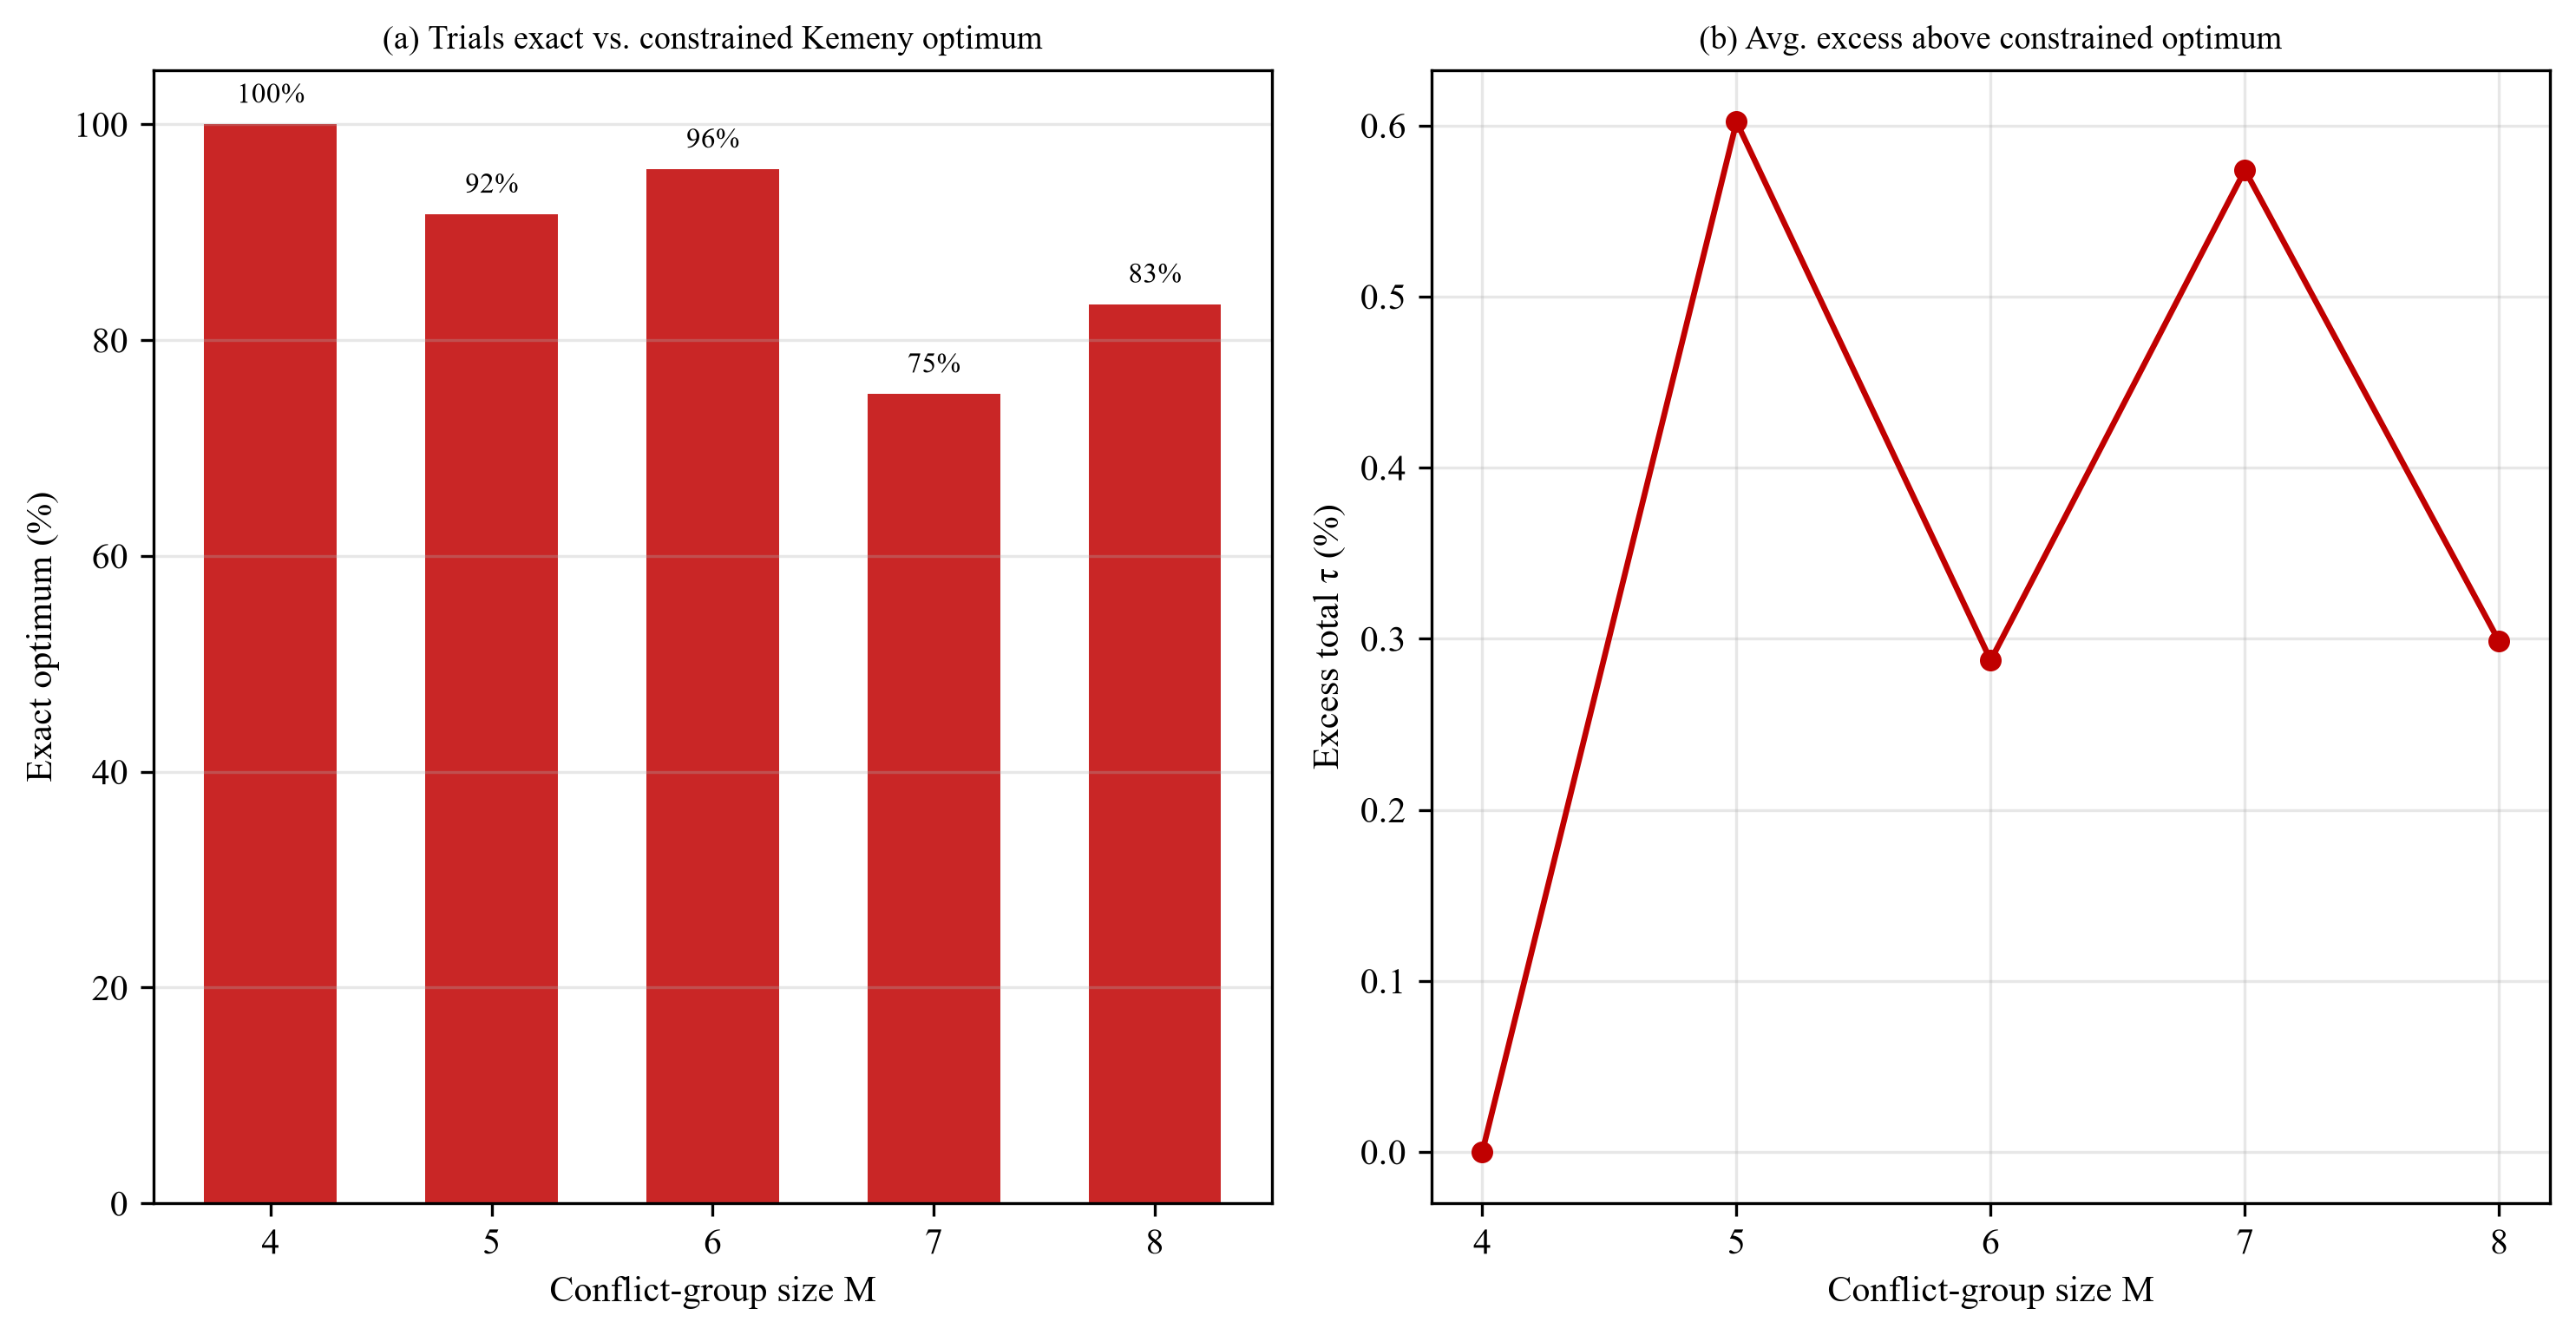
\includegraphics[width=0.95\textwidth]{figures/fig1.png}
\caption{Fig. 1. Validation that $\tau$-optimal feasible merging is achievable, via its concrete instantiation—the lexicographic (infinite-weight) case of weighted Ranked Pairs (causal edges locked first)—against the causally constrained Kemeny-Young optimum at small conflict-group sizes (N = 10, 24 trials each, partial ballots, no dissemination). (a) Fraction of trials in which the instantiation achieves the exact constrained optimum. (b) Excess total $\tau$ distance above the constrained optimum. The instantiation is exact in 89% of trials overall, with average excess 0.35% (maximum 8.0% in a single M = 5 trial); the constrained and unconstrained optima coincide in 100% of these trials.}
\end{figure}

The pattern confirms two properties. First, the weighting is nearly free: at high conflict the constrained optimum coincides with the unconstrained one in every trial, and the lexicographic instantiation matches it exactly in 89\% of trials with average excess $0.35%—\tau-optimal$ feasible merging operates at the theoretical frontier at negligible cost. Second, the hazard the weighting removes is real: on trace scenarios plain unweighted Ranked Pairs violates causal edges in 37.5\% of trials, while the weighted instantiation remains exact in 100\% of trials at every size (Table A1).

\subsection{Experiment 1: Causal Decomposition}
Proposition 2—the causal decomposition theorem—is the theoretical foundation of the metric. It states that total $\tau$ decomposes cleanly into $\tau_{\mathrm{causal}}$ and $\tau_{\mathrm{contested}};$ its feasibility corollary says any linear extension of the causal DAG contributes zero causal inversions. We therefore expect: (i) $\tau_{\mathrm{causal}}$ = 0 for every strategy that is causal-valid by construction (CF-RP, vector clocks, pure CRDT), while timestamp-based LWW/CRDT+LWW incur measurable causal violations under clock skew; and (ii) $\tau_{\mathrm{contested}}$ to rise as causal density falls, since fewer causally determined pairs means more genuinely contested pairs. Fig. 2 decomposes total $\tau$ distance at both conflict levels.

\begin{figure}[t]
\centering
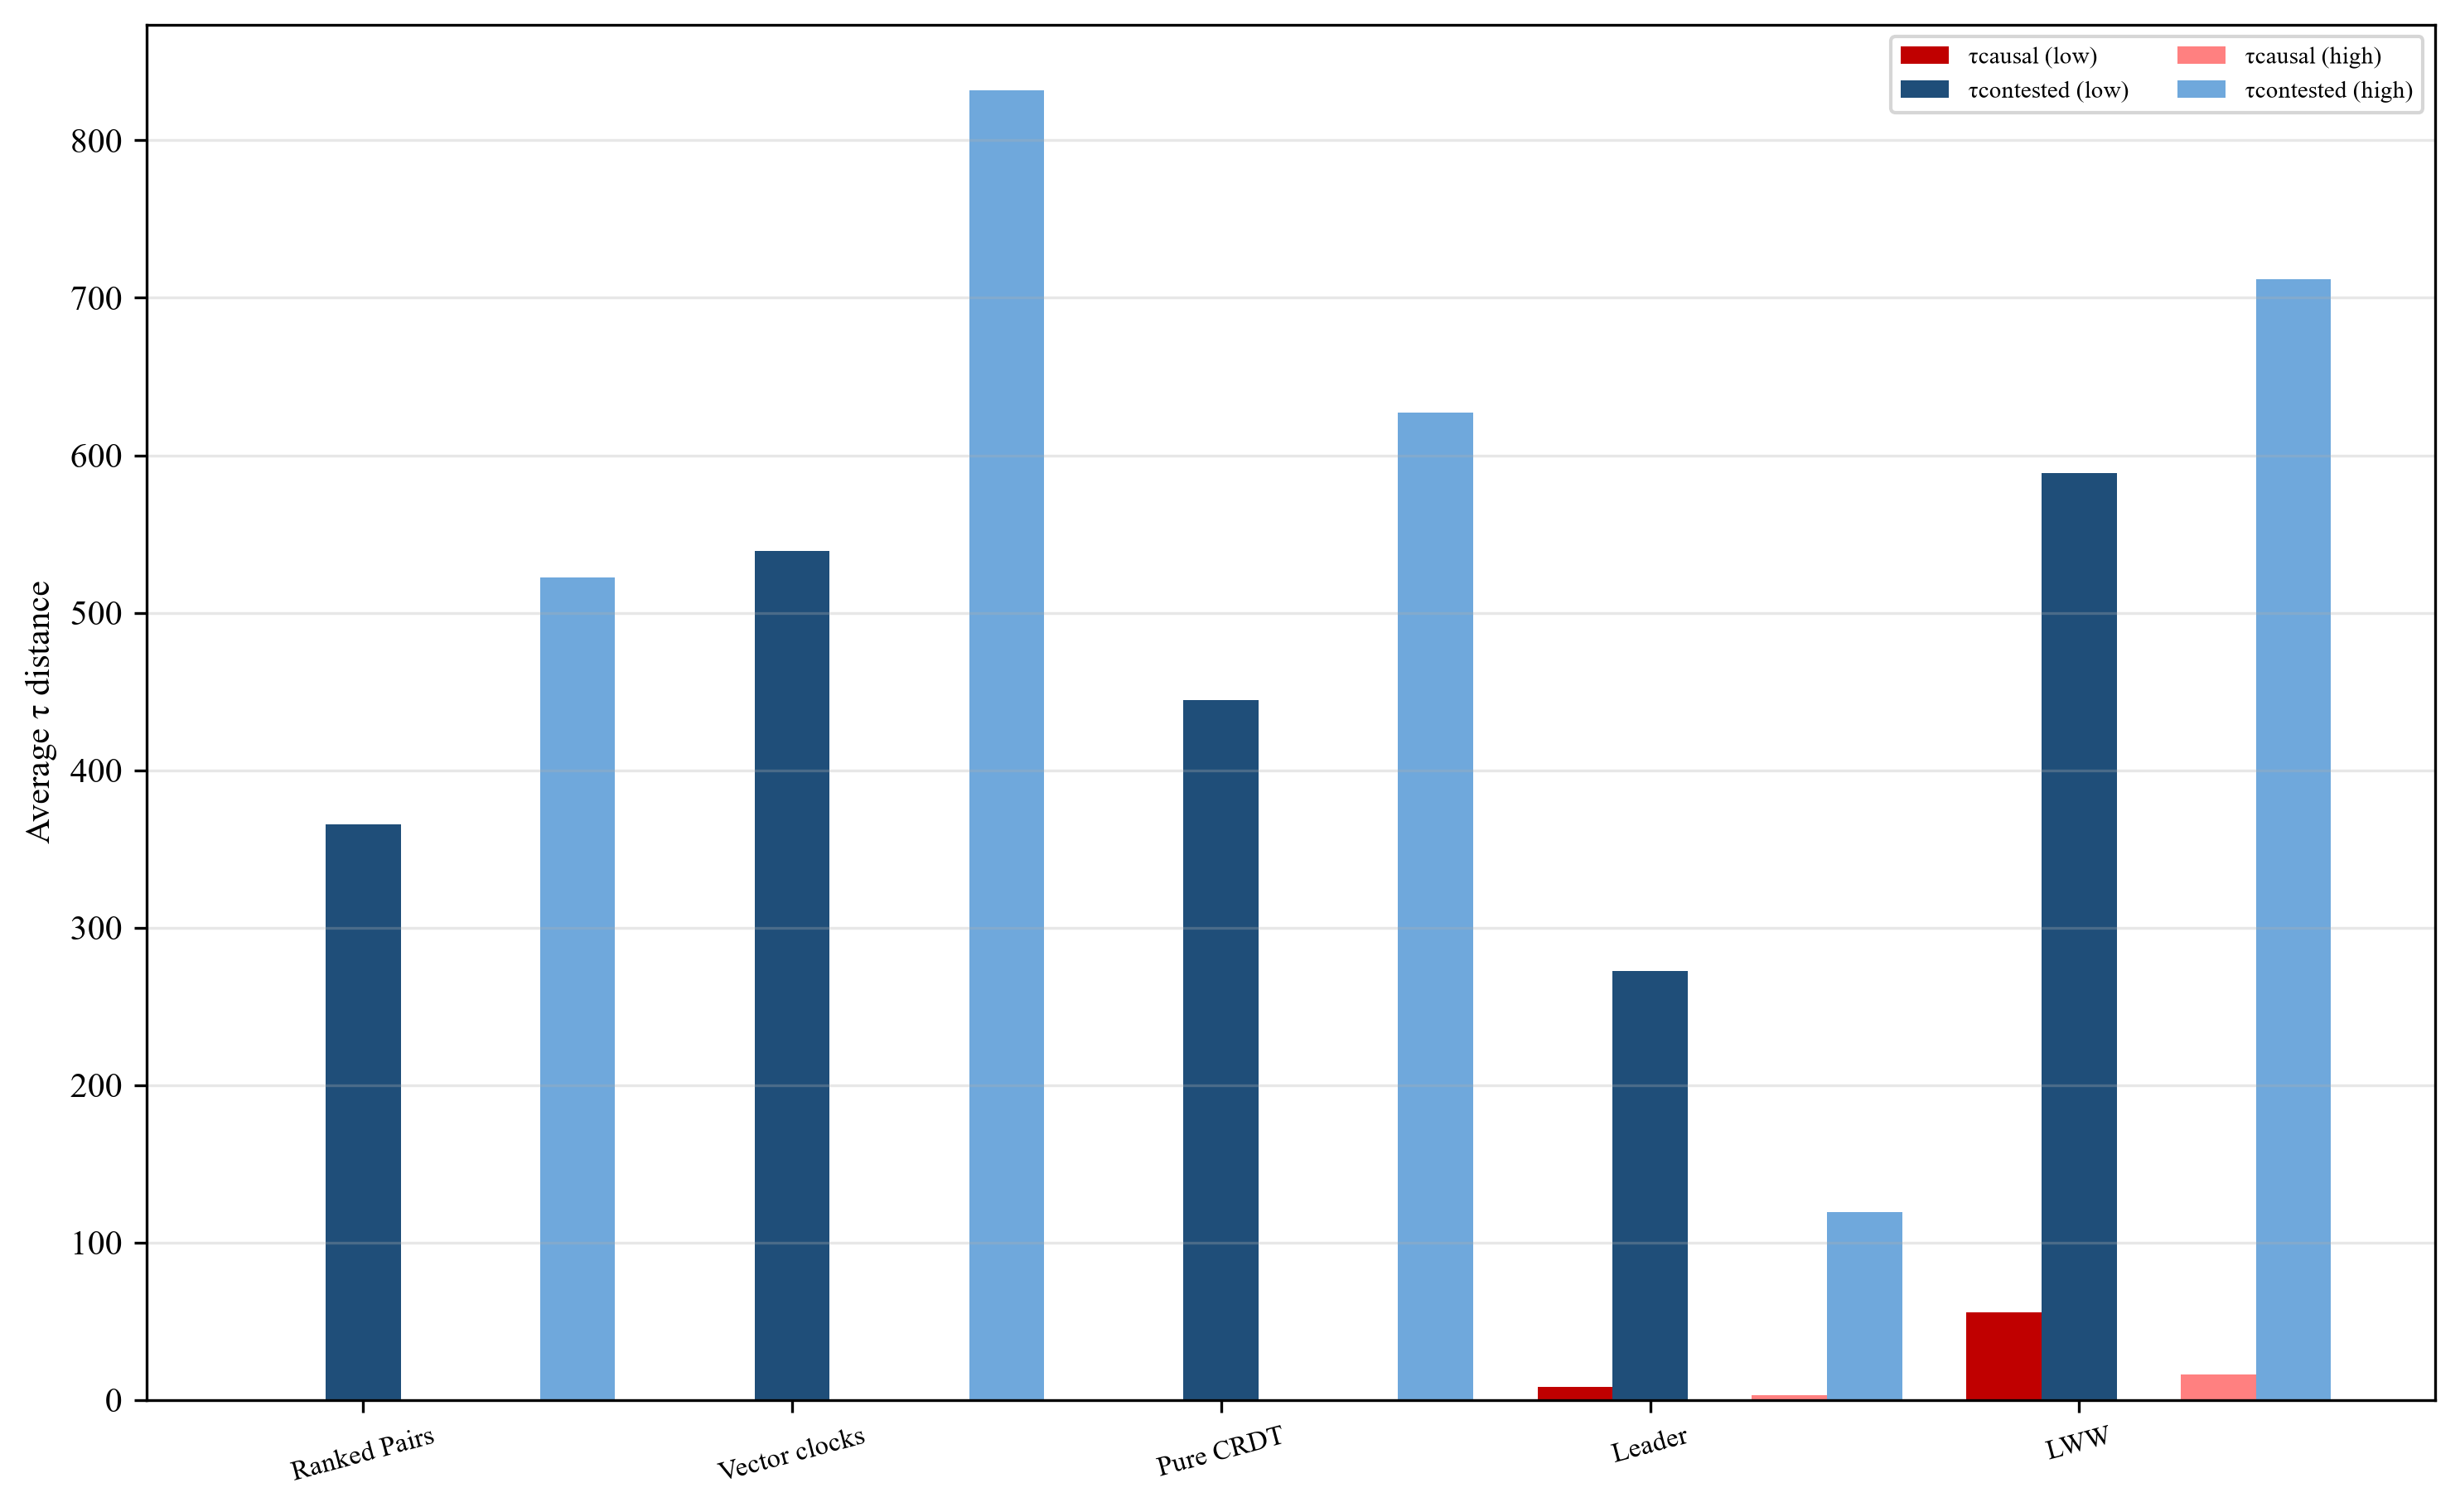
\includegraphics[width=0.95\textwidth]{figures/fig2.png}
\caption{Fig. 2. Causal decomposition of total $\tau$ distance (Proposition 2) on partial ballots without dissemination. Red: $\tau$_causal (causal-constraint violations). Blue: $\tau$_contested (genuine ordering disagreement). Dark bars: low conflict (35% causal density). Light bars: high conflict (10% causal density). $\tau$_causal is identically zero for CF-RP, vector clocks, and pure CRDT at both conflict levels—the constraint holds by construction—while timestamp-based LWW and CRDT+LWW incur 16.2 (high) to 55.3 (low) causal violations per trial on average, which the metric counts exactly; leader overwrite's timestamp-append fallback incurs 2.7–8.3.}
\end{figure}

Finding. Both predictions are confirmed under partial observation, with no dissemination. The constraint is exact: CF-RP, vector clocks, and pure CRDT achieve $\tau_{\mathrm{causal}}$ = 0 by construction; on these synthetic workloads unconstrained Ranked Pairs never violates a causal edge (identical outputs to CF-RP), so CF-RP's guarantee costs nothing here—though the hazard is frequent on traces (37.5\%, §7). Timestamp methods pay the skew price: LWW and CRDT+LWW incur 16.2 (high) to 55.3 (low) violations per trial, and $\tau_{\mathrm{contested}}$ rises by 21–54\% as causal density falls, confirming the two components are structurally distinct.

\subsection{Experiment 2: End-to-End Comparison}
We instantiate the trade-offs of §5.4 at high conflict—the regime where ordering disagreements are densest—and read the resulting $\tau$ values as quantified consequences of each design decision. Table 4 reports all dimensions; Fig. 3 visualizes the four principal axes.

\begin{table}[t]
\centering
\caption{Table 4. End-to-end reconciliation quality at high conflict (N = 10, M = 24, 15 trials, partial observation obs = 0.9, no dissemination).}
\begin{tabular}{lllllll}
\hline
Strategy & Ops ret. & Auto cov. & Info ret. & Caus. viol. & Sem. valid. & Time (ms) \\
\hline
Leader overwrite & 35.0\% & 100\% & 96.6\% & 1.0 & 100\% & 0.007 \\
LWW & 100\% & 100\% & 67.5\% & 14.4 & 74.9\% & 0.014 \\
Vector clocks & 100\% & 59.2\% & 61.3\% & 0.0 & 77.9\% & 0.047 \\
Pure CRDT * & 100\% & 59.2\% & 72.3\% & 0.0 & 72.8\% † & 0.022 \\
CRDT + LWW fb. & 100\% & 100\% & 67.5\% & 14.4 & 74.9\% & 0.012 \\
Ranked Pairs & 100\% & 100\% & 76.8\% & 0.0 & 87.0\% & 0.824 \\
\hline
\end{tabular}
\end{table}

* Pure CRDT resolves commutative operations perfectly; non-commutative concurrent writes are unresolved and require fallback. CRDT + LWW fallback uses LWW for unresolved registers, matching production CRDT libraries. † Semantic validity is the fraction of CAS operations that remain valid after merge, defined relative to each issuing replica's local state (no global ground truth assumed). ‡ Leader overwrite retains 35.0\% of operations (those issued by its 4-replica partition under a 4/3/3 split); its ordering retention (96.6\%) applies to the retained set, and its timestamp-append fallback incurs on average 1.0 causal violation per trial. All values are means over 15 partial-observation trials; standard deviations and confidence intervals in Table A5.

\begin{figure}[t]
\centering
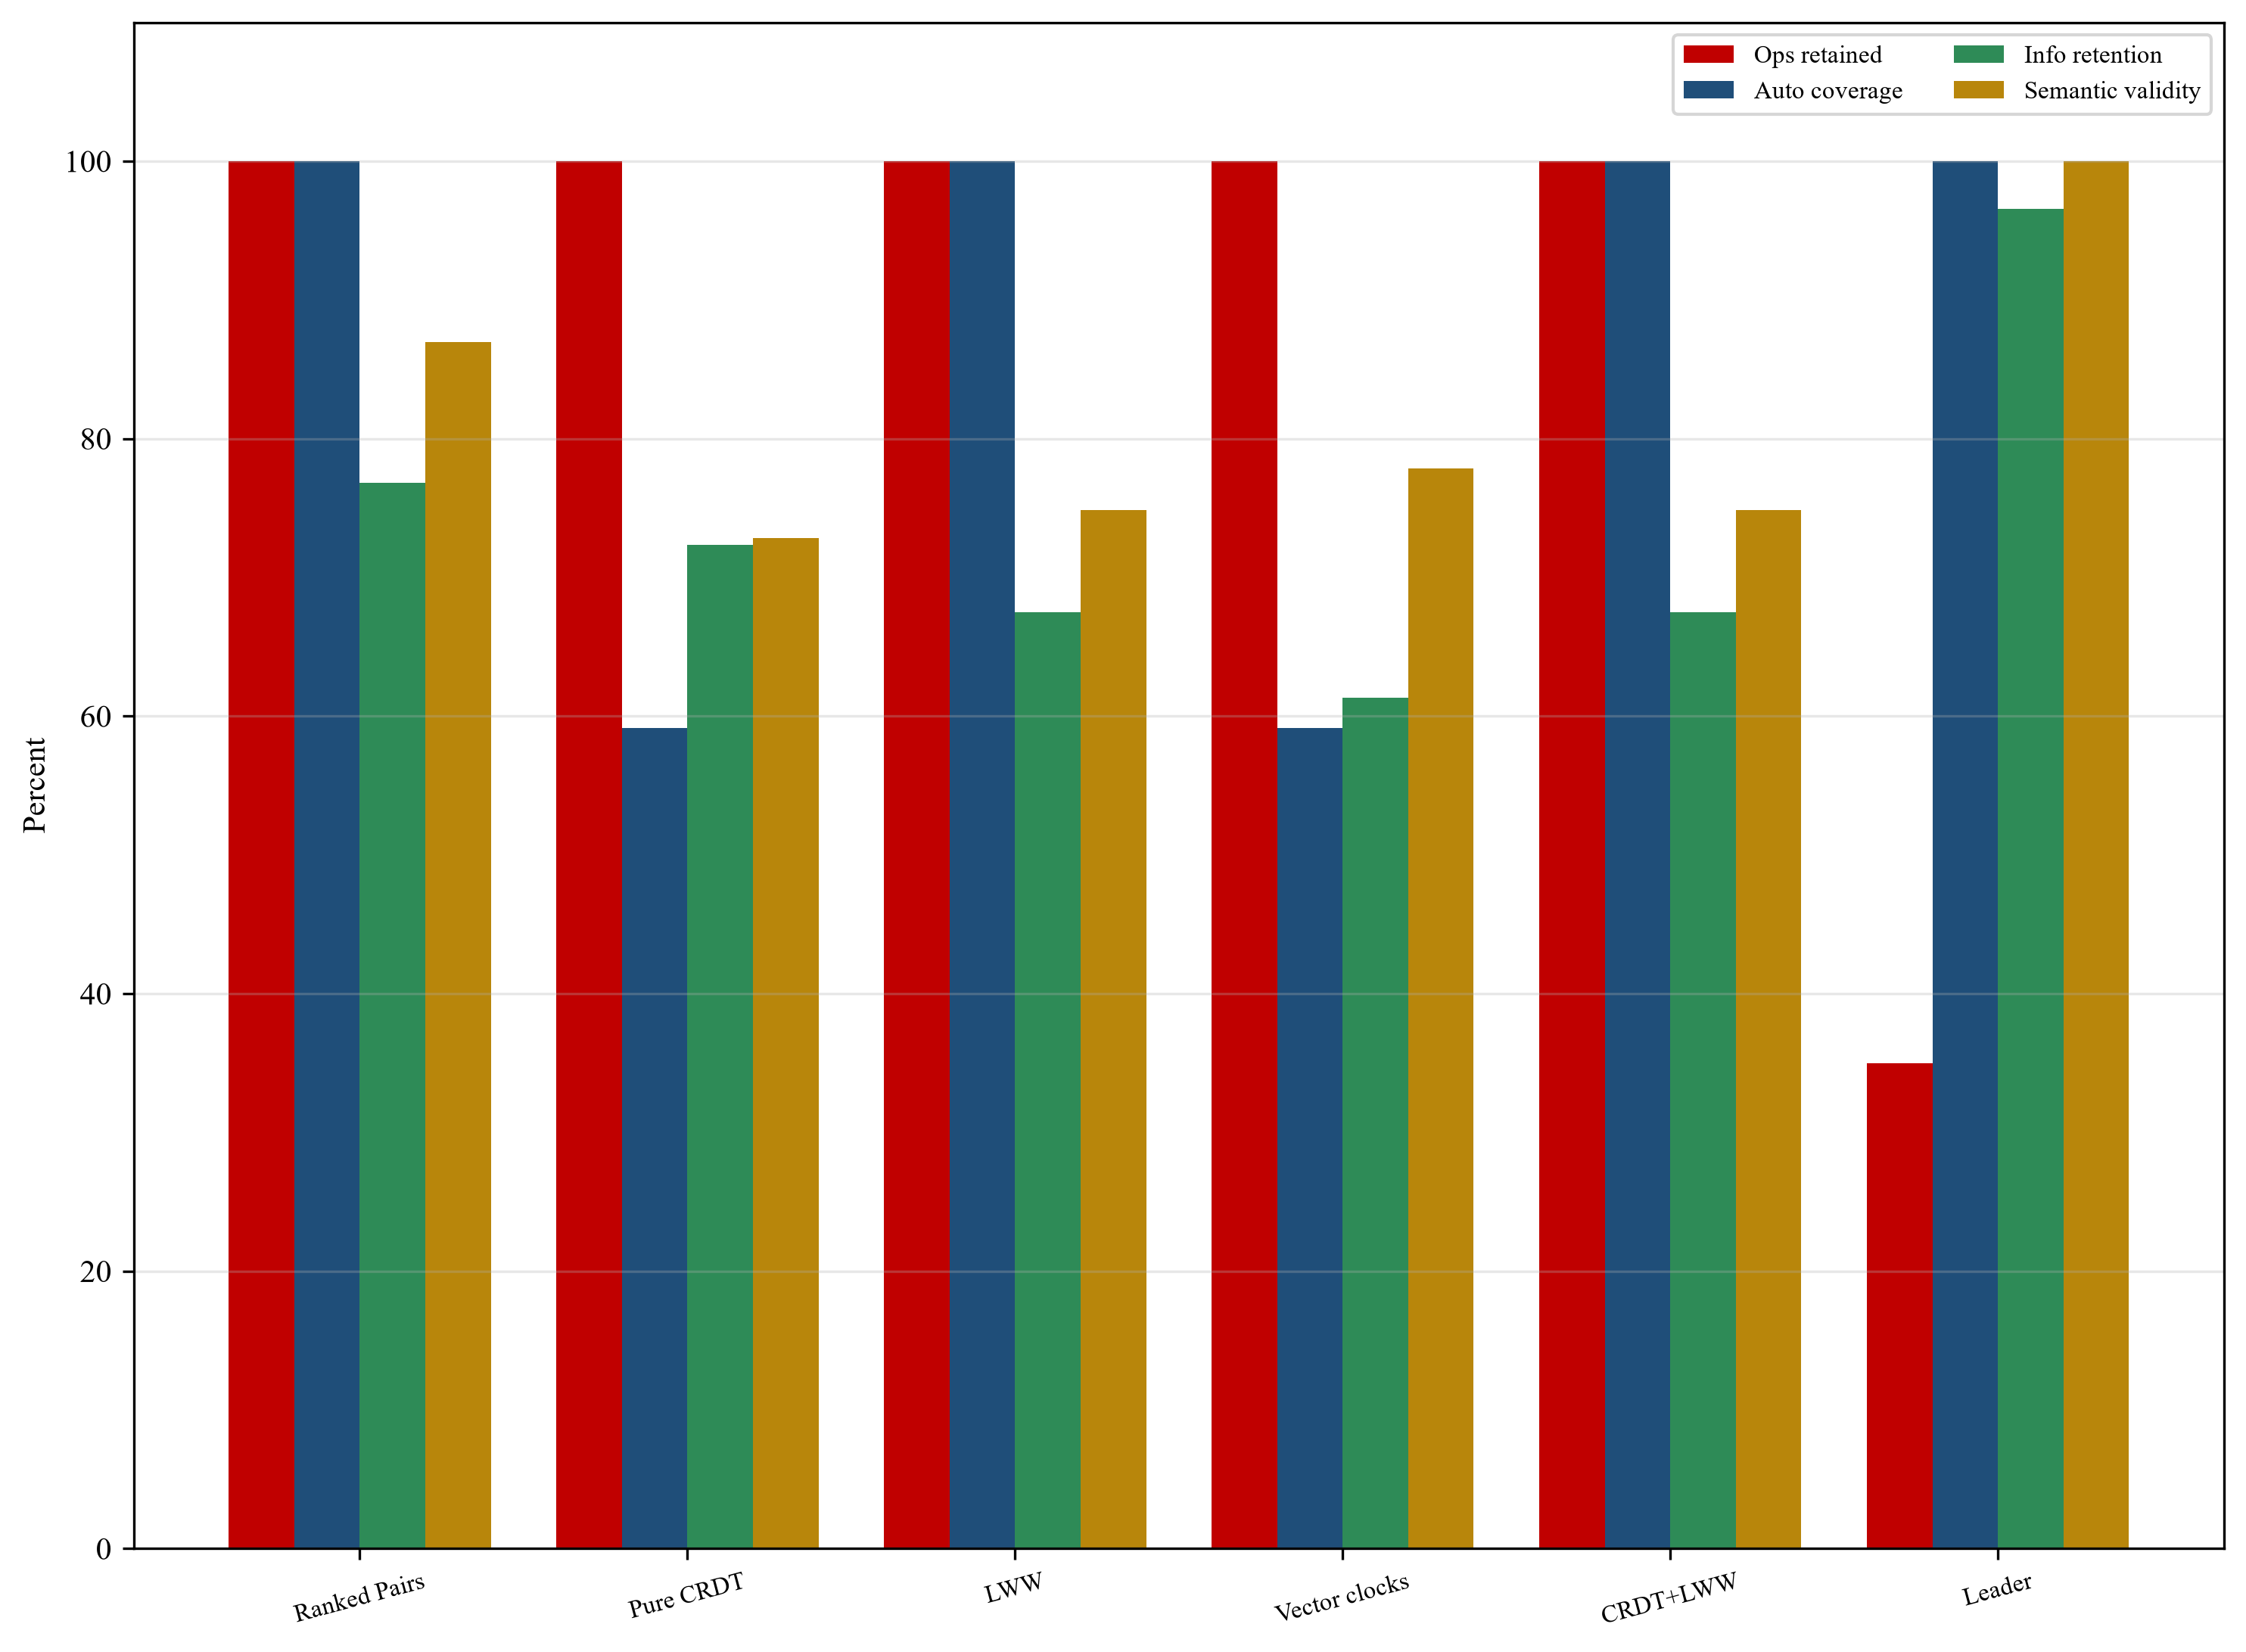
\includegraphics[width=0.95\textwidth]{figures/fig3.png}
\caption{Fig. 3. End-to-end quality at high conflict under partial ballots (no dissemination). Each design decision materializes as a quantified cost on the four axes: leader overwrite retains 35.0% of operations; LWW keeps 67.5% of ordering information and violates 14.4 causal constraints on average; vector clocks automate 59.2% of resolutions and keep 61.3%; pure CRDT covers 59.2%; CRDT+LWW fallback covers everything at LWW quality; CF-RP retains 76.8% of ordering information with zero causal violations and full automation.}
\end{figure}

Findings. Read as quantifications of each method's design decision—not as a ranking—the numbers expose the concrete benefit and the concrete cost each decision carries in its intended domain:

Leader overwrite's retention law is the observable price of linearizability: under a 4/3/3 partition, 65.0\% of operations are truncated—a cost that scales linearly with minority share (§6.6, 90\% $\rightarrow$ 51\%). The benefit is that the surviving 35.0\% keeps 96.6\% of its ordering information; the consequence is that \emph{information loss is a design constant, not a failure mode}—the designer who accepts consensus ordering must budget a precisely predictable loss.

LWW's trade-off quantifies the price of zero coordination: it retains 100\% of operations at no communication cost, but its externally decreed order keeps only 67.5\% of the ordering information in the adversarial regime, and under realistic clock skew it injects 14.4 causal violations per trial that $\tau_{\mathrm{causal}}$ detects exactly. The engineering consequence is directional: LWW is the right choice when the contested mass is small or commutativity is high (§6.5 shows its $\hat{\tau}$ approaches the unconstrained ceiling there), and its clock-skew risk becomes auditable—if causal violations appear in monitoring (§7), the deployment should revisit skew bounds rather than the LWW choice itself.

Vector clocks buy perfect causal information (zero violations) and defer everything else; the measure of that deferral is the 15-point retention gap to majority aggregation (61.3\% vs. 76.8\%) and the 41-point automation gap (59.2\% coverage). The consequence for practice is that VC is the instrument of choice precisely when application-level arbitration exists—rich merge policies in multi-master editing—because it preserves the information those policies need; when no such policy exists, the deferred mass is resolved by entropy, a cost VC's design decision makes explicit but cannot prevent. At low conflict the random-tie-breaking penalty narrows (76.2\% vs. 71.7\% for LWW), confirming the cost scales with contested density only.

Pure CRDT's boundary is the semantic-validity guarantee: within its commutative domain it is optimal by construction (100\% valid), and its 59.2\% coverage at high conflict is simply the residual share of commutative operations in that workload. The consequence is a design rule rather than a verdict: the interesting quantity is the non-commutative share of \emph{your} workload—Fig. 4 (§6.5) gives the coverage-vs-share curve—from which the operator reads directly whether a CRDT model suffices or whether the fallback path (LWW) will dominate behavior.

The $\tau$-minimizing decision (CF-RP) spends $O(M^{2}$ log M) local computation—and no communication—to recover the contested mass that the other decisions forgo: 76.8\% retention, zero causal violations by construction, and full automation, significantly above every alternative at $\alpha$ = 0.05 (§6.9). Its cost curve (§6.7) is sub-millisecond for realistic groups, so the trade-off is favorable wherever ordering quality has business value—audited logs, merge hubs, fair-ordering pipelines—and its only input requirement beyond the ballots is the version-clock metadata the ballots already carry (§4.1).

The \emph{parameter} driving these numbers is causal density: as conflict falls from high to low, the contested mass shrinks and the gaps compress—CF-RP retains 83.9\% vs. 71.7\% for LWW at low conflict—while vector clocks overtake LWW (76.2\% vs. 71.7\%) because random tie-breaking loses less with fewer contested pairs. What is stable across regimes is the \emph{direction of each mechanism's cost}; the designer needs to know what each decision costs as the workload changes, not which method wins.

\subsection{Experiment 3: The CRDT Ceiling and Its Applicability Boundary}
CRDTs represent the theoretical ceiling for automatic reconciliation: where operations commute, order is semantically irrelevant and convergence is guaranteed. How broad is this ceiling, and how sharply does it break down as non-commutative operations enter? We sweep the non-commutative fraction from 0\% to 100\% under high conflict, comparing pure CRDT, CRDT with LWW fallback, LWW, and Ranked Pairs, quantifying where the ceiling ends and what quality the fallback provides.

\begin{figure}[t]
\centering
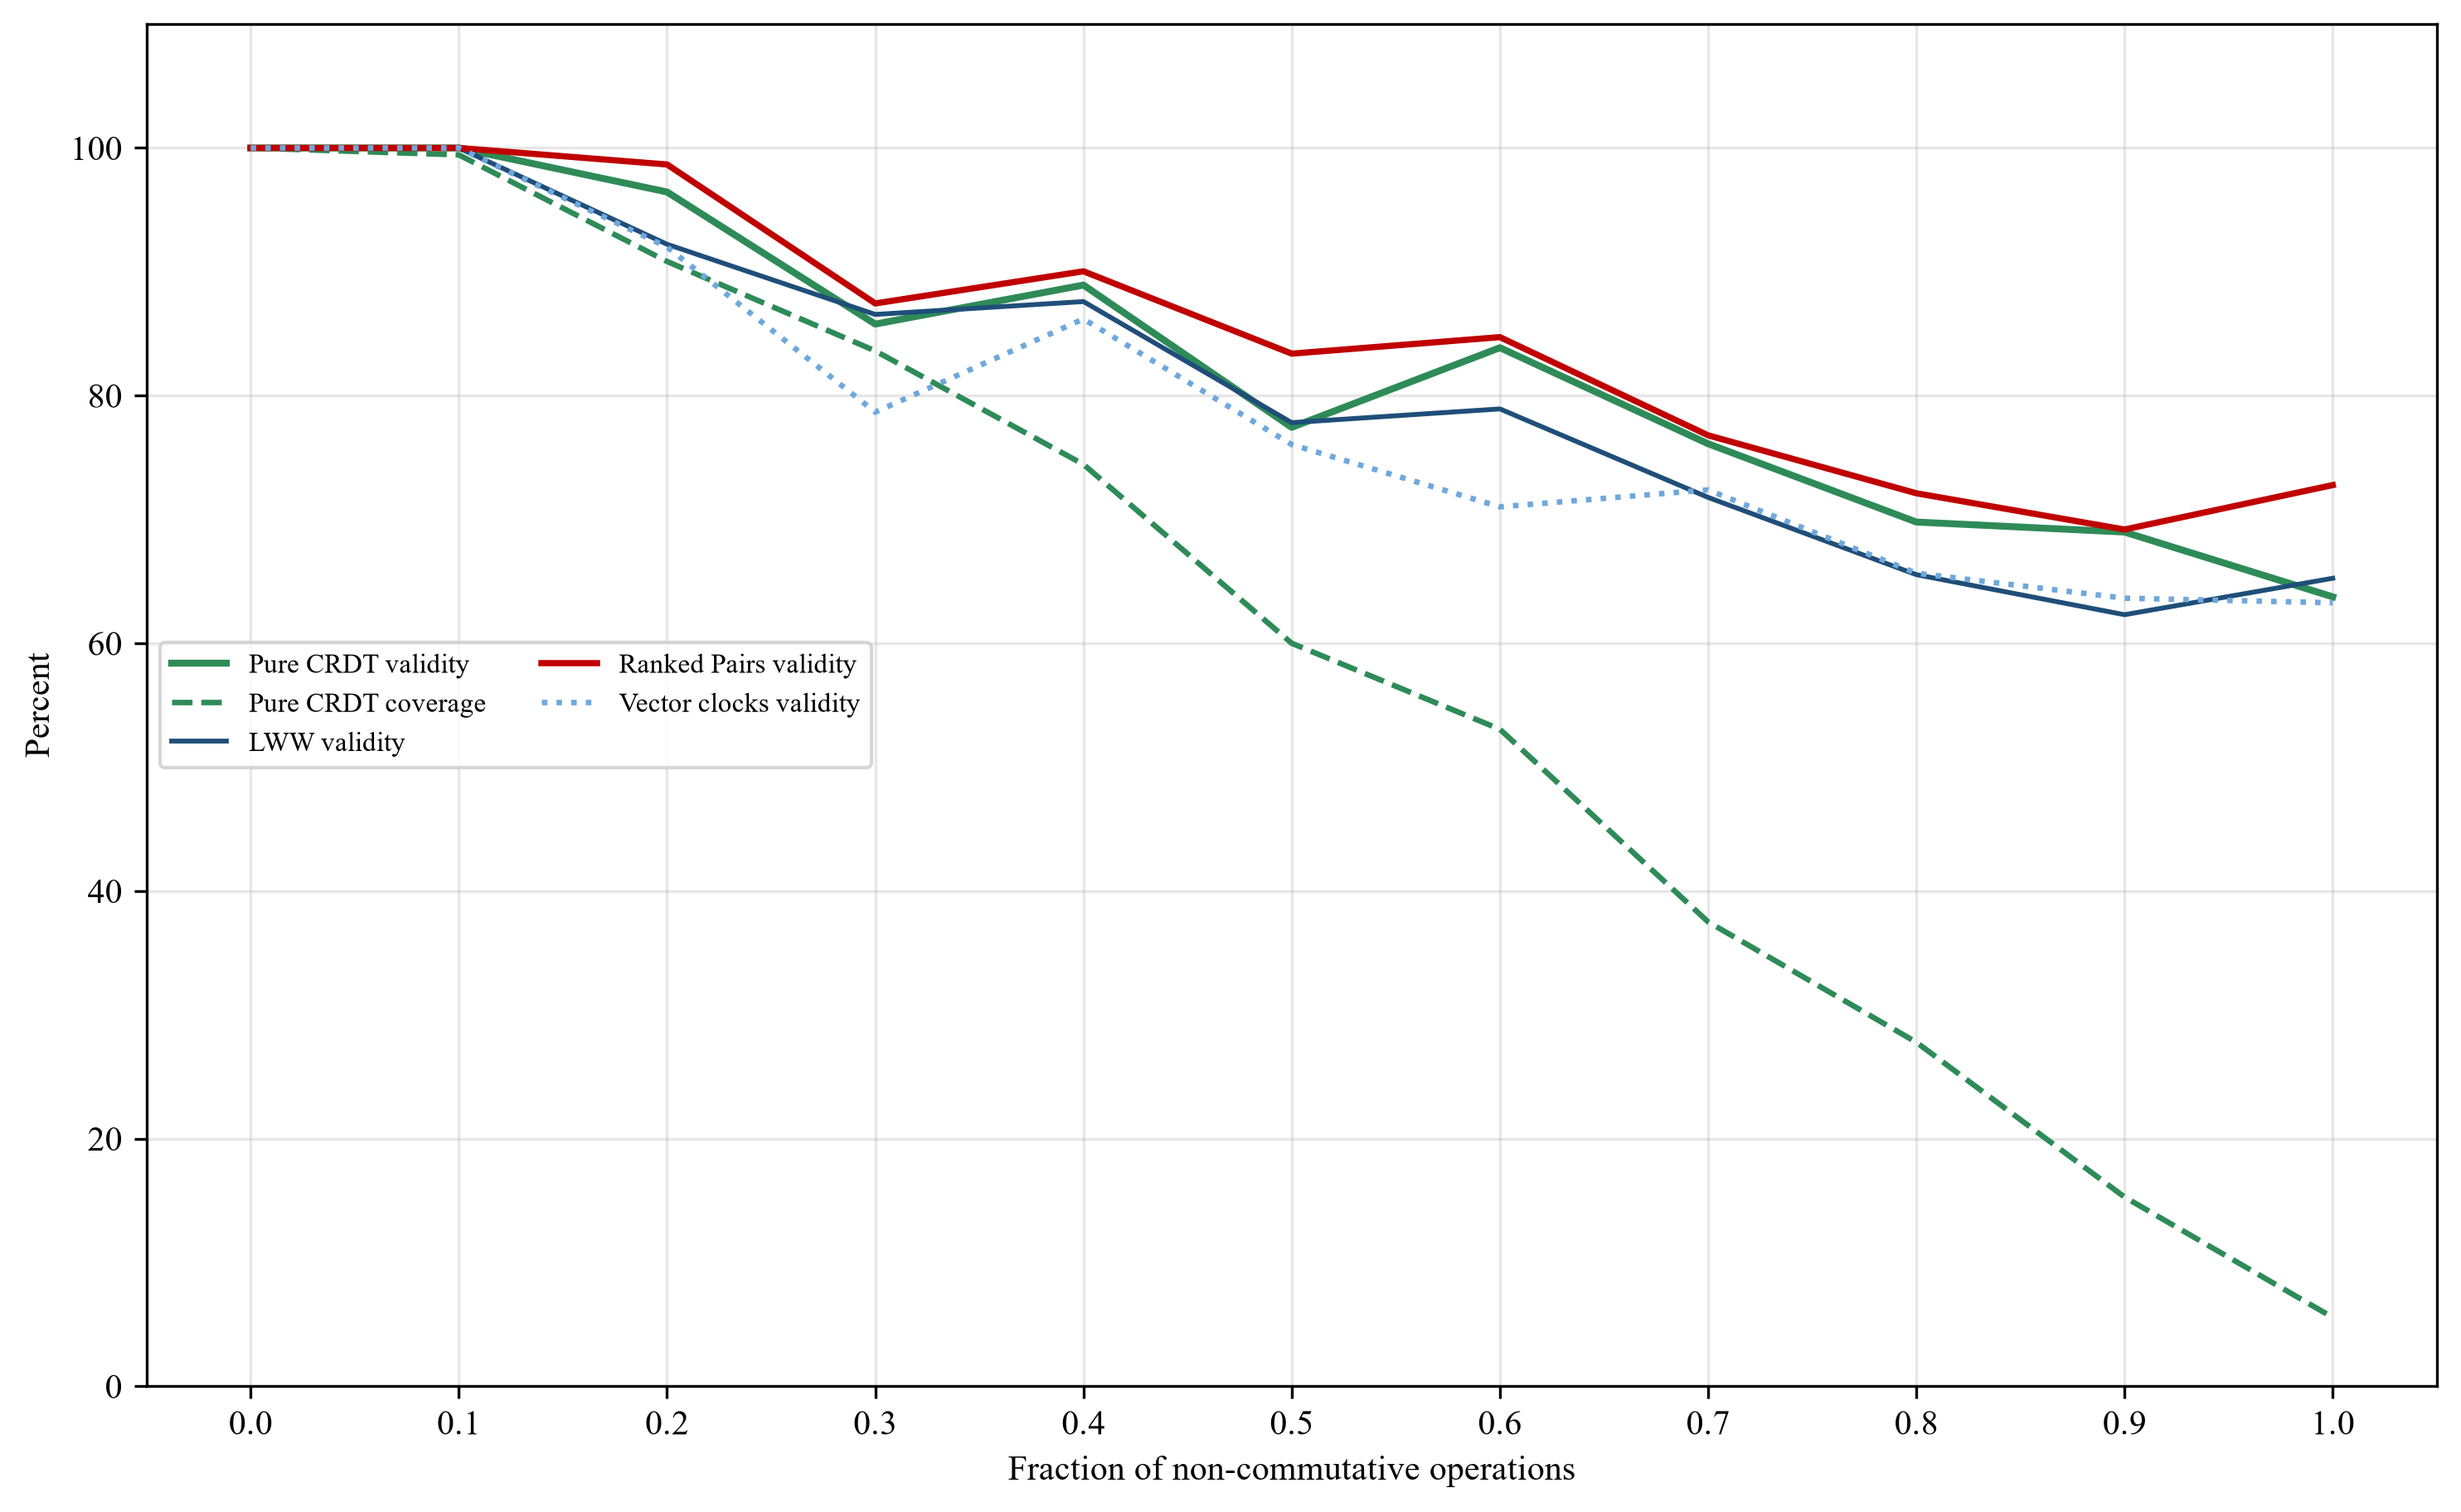
\includegraphics[width=0.95\textwidth]{figures/fig4.png}
\caption{Fig. 4. Semantic validity versus non-commutative operation fraction (partial ballots, 15 trials per point, no dissemination). Pure CRDT (solid green) maintains near-100% validity at low non-commutative fractions, but its automatic coverage collapses from 100% to 5.6% (dashed green line) as the non-commutative fraction reaches 100%. CRDT + LWW fallback (dark green dash-dot) keeps 100% coverage while validity drops to LWW levels. Ranked Pairs (red) holds 100% coverage with the highest validity among automatic methods at high non-commutative fractions; VC (light blue dotted) trails on both axes.}
\end{figure}

Finding. The pure CRDT ceiling is real but narrow: automatic coverage of perfect semantics falls to 91\% once one operation in five is non-commutative, and to under 28\% once four in five are non-commutative (5.6\% in the fully non-commutative limit). Production CRDT libraries implicitly concede this by backing maps and registers with LWW—that is, they fall back to timestamp-ordered resolution. The CRDT+LWW configuration achieves 100\% coverage but at LWW-level validity (dropping to 65\% at high non-commutative fractions), consistent with the design-space characterization. Ranked Pairs provides a middle ground: full coverage, the highest validity among automatic methods at high non-commutative fractions (73\%), and no type restrictions. The $Kendall-\tau$ objective is, in effect, a generalization of the CRDT guarantee from \emph{order must not matter} to \emph{order disagreements are resolved by majority evidence.}

\subsection{Experiment 4: Data Preservation Under Partition Asymmetry}
The cost of leader-based overwrite is usually described qualitatively ('minority writes are lost'). Kendall $\tau$ lets us quantify this information loss precisely, because operation loss and ordering loss are both pairwise-information losses measured on the same scale. We sweep the minority partition size from 10\% to 50\% of replicas, with operations arriving in proportion to partition size.

\begin{figure}[t]
\centering
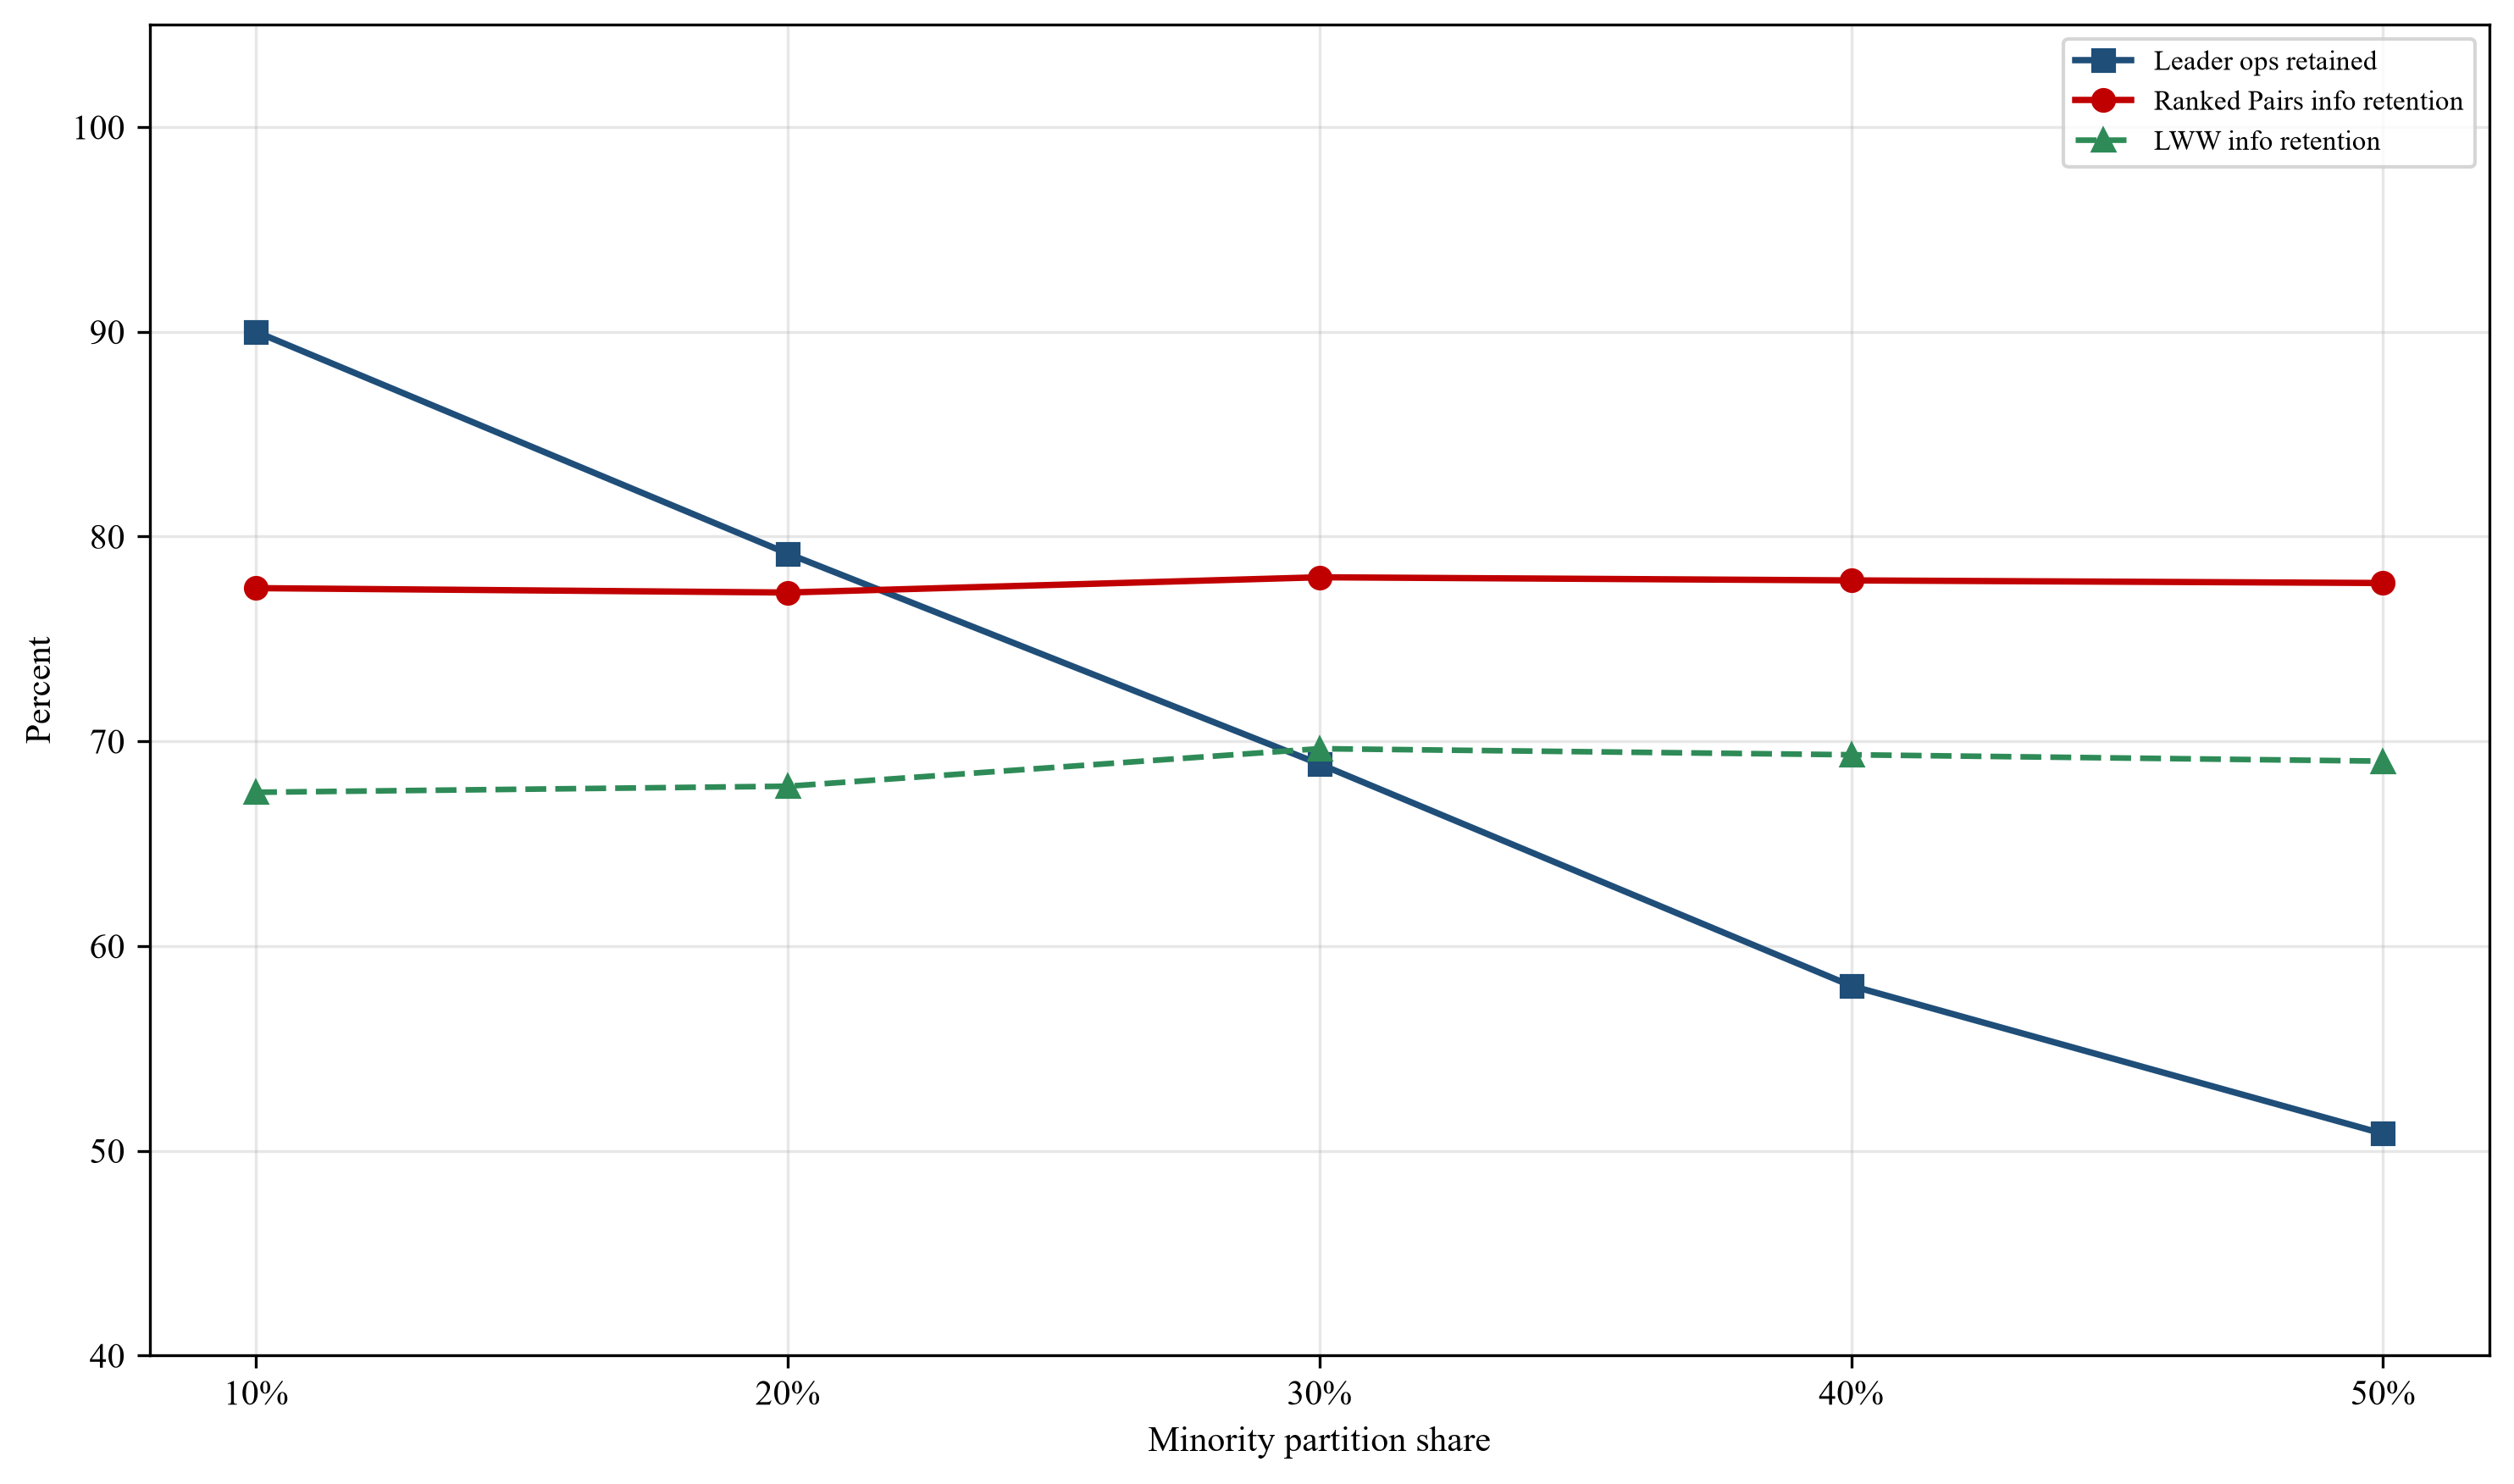
\includegraphics[width=0.95\textwidth]{figures/fig5.png}
\caption{Fig. 5. As the minority partition grows, leader-based overwrite retains fewer operations (90% $\rightarrow$ 51%). Full-retention strategies (LWW, CF-RP) stay flat on ordering information retention, with CF-RP consistently 8–10 percentage points above LWW.}
\end{figure}

Finding. Leader-overwrite operation retention tracks majority size one-for-one (90\% $\rightarrow$ 51\% as minority grows from 10\% to 50\%), and $\tau$ on surviving operations remains low—consistent with the element-set-removal mechanism described in §5.4. Full-retention strategies (Ranked Pairs, LWW) are flat on ordering information retention across the sweep, with CF-RP consistently 8–10 percentage points above LWW (77.3–78.0\% vs. 67.5–69.6\%). The normalized $\tau$ metric captures this distinction directly: operation loss and ordering loss are both pairwise-information losses, measured on the same scale. On the trace platform the conservative leader-log implementation retains 88\% $\rightarrow$ 50\% of operations over the same sweep (Appendix A), preserving the monotonic trend.

\subsection{Computational Cost}
\begin{figure}[t]
\centering
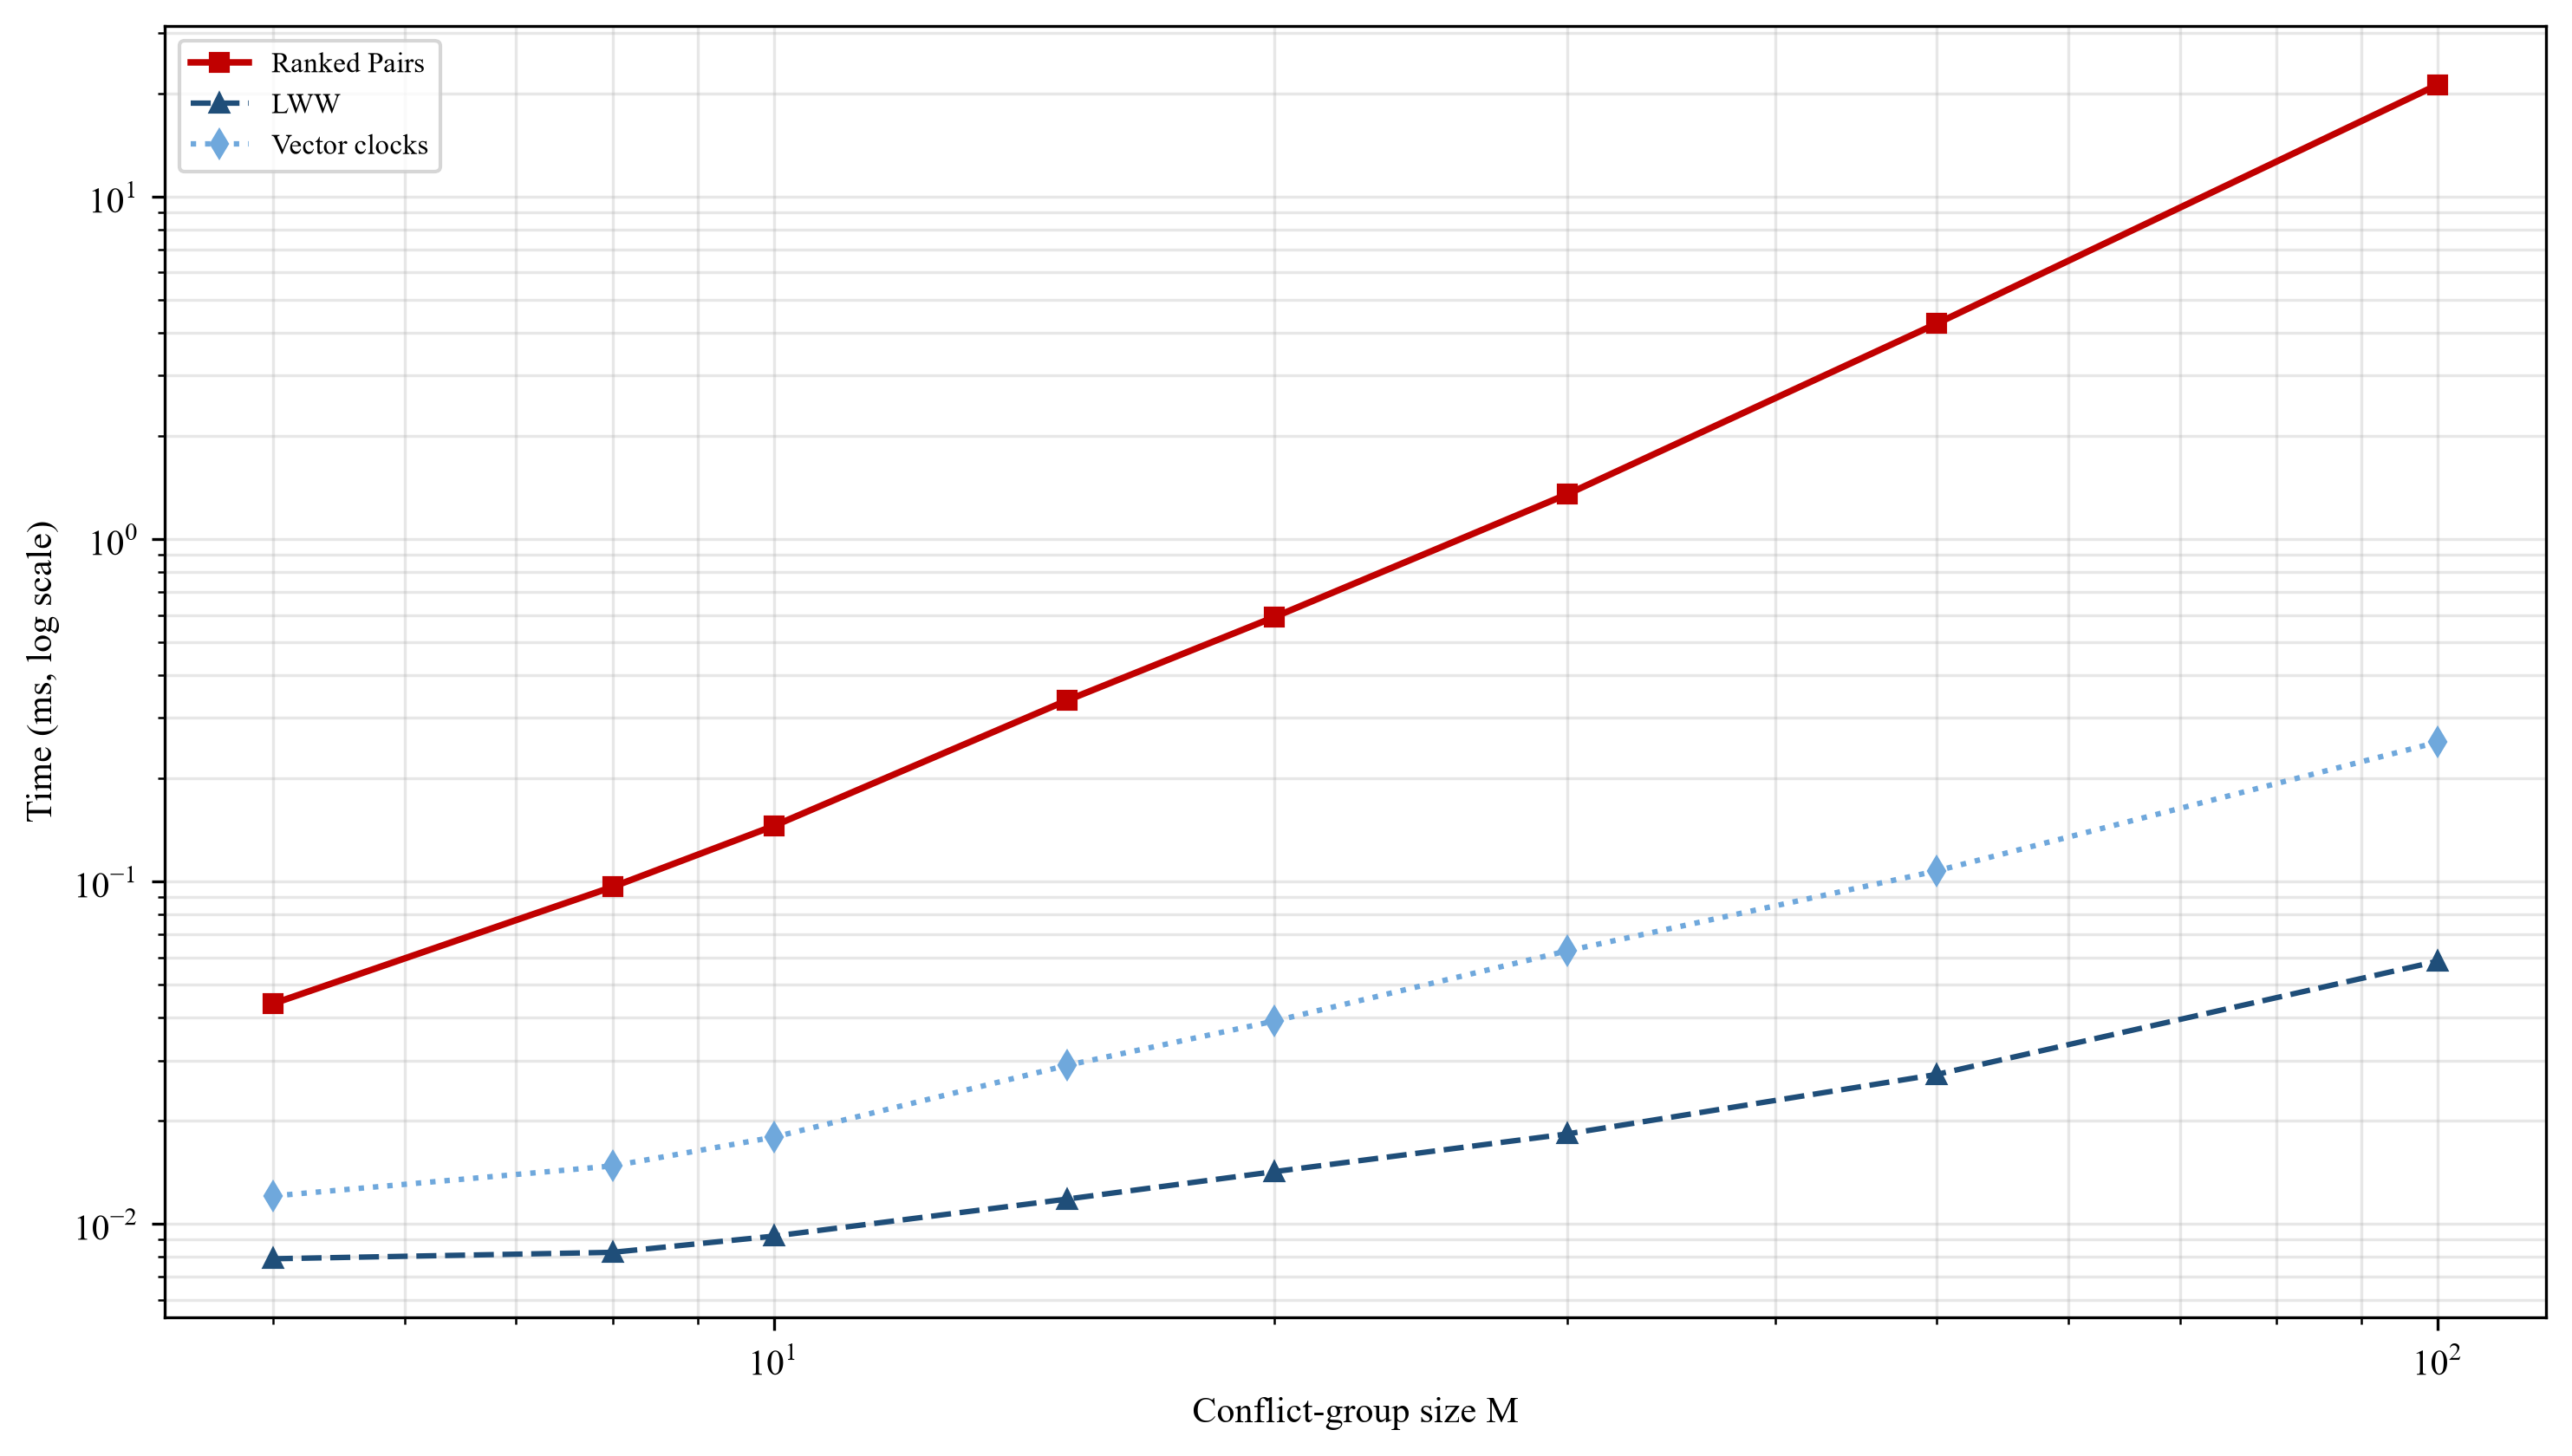
\includegraphics[width=0.95\textwidth]{figures/fig6.png}
\caption{Fig. 6. Reconciliation time versus conflict-group size (log scale) on partial ballots. CF-RP is sub-millisecond for typical groups (M $\leq$ 20), 1.35 ms at M = 30, 4.4 ms at M = 50, and $\approx$21 ms at M = 100—an extreme case; causal pre-locking adds no measurable overhead over plain Ranked Pairs. LWW and VC detection are cheaper but produce the quality losses measured above.}
\end{figure}

Finding. CF-RP reconciliation costs 0.15 ms at M = 10, 1.35 ms at M = 30, and 21.4 ms at M = 100 (single-threaded Python, partial ballots); the causal pre-locking phase is absorbed into the margin computation and adds no measurable cost over plain Ranked Pairs. The guarantee is therefore bought with $O(M^{2}$ log M) local computation alone—no dissemination, no extra communication—and conflict groups in practice are small (most divergent operations are causally ordered and fast-forwarded), so the typical cost is sub-millisecond. The overhead relative to LWW is the price of recovering the contested mass plus an unconditional causal guarantee.

\subsection{Summary}
Kendall tau distance proves to be a discriminating and informative quality metric for log reconciliation. It reveals the structure of the design space:

Causal decomposition is real. Total $\tau$ cleanly separates into causal and contested components (§6.3): constructively causal-valid strategies keep $\tau_{\mathrm{causal}}$ = 0, and $\tau_{\mathrm{contested}}$ grows by 21–54\% as causal density falls from 35\% to 10\%.

$\tau$-optimal is practically achievable with local computation only: CF-RP reaches the constrained Kemeny-Young optimum in 89\% of synthetic trials (avg. excess 0.35\%, §6.2) and 100\% of trace trials (§7); causal validity comes from the constraint set, unconditionally over partial ballots.

Each design decision carries a quantifiable, mechanism-specific cost: truncation loss is set by partition asymmetry (§6.6), LWW's retention loss by contested density, VC's deferral penalty is per undeclared pair, CRDT's boundary by the non-commutative share (§6.5), and $\tau-aggregation's$ cost is $O(M^{2}$ log M) of local computation (§6.7)—a parameterized menu, not a single winner.

The CRDT ceiling is narrow: automatic coverage collapses from 100\% to 5.6\% as the non-commutative share reaches 100\%, and below 28\% once four in five operations are non-commutative; production CRDTs fall back to LWW-quality ordering there (§6.5).

Leader-overwrite loss is quantifiable. Operation retention tracks majority partition size one-for-one, confirming the element-set-removal mechanism of §5.4. The $\tau$ metric puts operation loss and ordering loss on the same scale (§6.6).

Causal validity for CF-RP is unconditional: locking causal edges before majority aggregation makes the output a linear extension of causal order for arbitrary partial ballots (Proposition 4(a))—no dissemination, no constraint checking. Unconstrained aggregation retains the hazard: plain Ranked Pairs violates causal edges in 37.5\% of trace trials (§7), which the constraint removes at zero quality cost; timestamp LWW violates causal constraints under clock skew (14.4–55.3 per trial), which $\tau$ counts exactly.

\subsection{Statistical Reliability}
All statistics are computed per-trial over paired inputs: within each trial, every strategy consumes byte-identical scenarios, so the observations are paired and significance can be tested without independence assumptions across trials. Means are reported with standard deviations; 95\% confidence intervals use the t distribution with n $-$ 1 degrees of freedom (n = 15 synthetic, n = 30 trace); pairwise strategy significance is tested with the two-sided paired Wilcoxon signed-rank test at $\alpha$ = 0.05, with ties (identical outputs, e.g., LWW and CRDT+LWW) reported as p = 1.0. Detailed per-metric tables for E1/E2/E6a are given in Appendix A.5.

On the synthetic platform (Table A5), CF-RP retains 76.8 $\pm$ 2.7\% of ordering information, significantly more than LWW (67.5 $\pm$ 3.7\%, p < 0.001), vector clocks (61.3 $\pm$ 5.1\%, p < 0.001), and pure CRDT (72.3 $\pm$ 3.3\%, p < 0.001); its advantage over every automatic method is significant at $\alpha$ = 0.05, with disjoint 95\% confidence intervals. LWW and CRDT+LWW produce identical outputs on every trial (p = 1.0). On the trace platform (Table A6) CF-RP recovers the exact consensus order on every trial (100.0 $\pm$ 0.0\%), significantly above LWW and pure CRDT (99.0 $\pm$ 1.7\%, p = 0.008) and vector clocks (68.4 $\pm$ 8.7\%, p < 0.001), while leader overwrite trades away 39.3\% of operations for 99.5 $\pm$ 1.2\% retention on the surviving set; unconstrained Ranked Pairs on the same ballots violates causal edges in 37.5\% of validation trials (Table A1). The Wilcoxon tests confirm that the quantitative conclusions of §6.4 hold with statistical reliability.

\section{Validation on Real Traces}
\subsection{The Monitoring System and Scenarios}
\subsection{Monitor design. The monitoring system runs as a coordinator-side process that samples the per-replica logs at a fixed period (1 s in our deployment) and maintains a sliding window over the most recent operations of each replica. For each window it computes the merged $\hat{\tau}$ of §5.1 with effective normalization—Z\_eff accounts for live windows that do not yet contain all operations, so the measure stays calibrated under partial observation—and compares it against two standard signals: the maximum replica lag (a binary, set-level indicator) and the operation-set Jaccard index (a similarity indicator). An alert fires when windowed $\hat{\tau}$ crosses a threshold that no benign steady-state fluctuation reaches. The design is deliberately light: no coordination, no propagation, and no instrumentation beyond reading the logs; per-window cost is O(M² log M) in the window size, negligible at production sampling rates.}
The workloads of §6 are synthetic by design: partition balance, causal density, and clock skew are controlled to expose worst-case disagreement, so the magnitudes of the strategy gaps are properties of the generator. To test the theory on data we did not construct, we re-run the full measurement suite of §6 against scenarios built from real system logs and deployed on a four-node Cassandra 4.1 cluster (RF = 2) containerized with Docker Compose on a single host. We use the BGL log (Blue Gene/L, Lawrence Livermore National Laboratory) as the primary trace and the HDFS log (Hadoop) as a cross-check, both from the Loghub collection [44], [45]. Each log line is mapped to a typed operation under the semanticization of §6.1; a causal DAG is built to the target density, and each replica's local log is a causally consistent subsequence (mapping and platform details in Appendix A). Scenarios are materialized on a four-node Cassandra 4.1 cluster (RF = 2) deployed with Docker Compose; a Python coordinator reads per-replica logs, runs all six strategies on identical inputs, and evaluates the §6.1 metrics. Defaults match §6.1 with N = 8 logical replicas, M = 24, 30 trials, and fixed seed 42.

\subsection{Results: Monitoring and Merge Validation}
Every qualitative prediction of the theory survives on real traces under partial observation. The causal decomposition is exact: $\tau_{\mathrm{causal}}$ = 0 across all trials and strategies; CF-RP (our validation instantiation; the infinite-weight limit of weighted Ranked Pairs, §9.4.1) matches the constrained Kemeny-Young optimum in 100\% of trials (Table A1) and recovers the consensus order exactly (100.0 $\pm$ 0.0\%), because the trace's single-source timestamps are internally consistent; LWW and CRDT follow at 99.0 $\pm$ 1.7\% (p = 0.008), vector clocks fall to 68.4 $\pm$ 8.7\% (p < 0.001), and leader overwrite retains 60.7\% of operations with 99.5\% retention on the surviving set. The new result is the hazard the constraint removes: unconstrained Ranked Pairs violates causal edges in 37.5\% of trials (9.1 edges/trial), invisible to ballot-weighted $\tau_{\mathrm{causal}}$ because no replica co-observed those pairs—undetectable without the metadata check. CF-RP eliminates this hazard by construction at zero quality loss.

The most informative new result is the monitoring system of §7.1 in operation, providing the first direct confirmation that $\tau$ detects ordering divergence that binary lag and operation-set similarity cannot. During an in-place ordering drift—an intentional reshuffling that adds no new $operations—\hat{\tau}$ rises from 0 to 0.31–0.43 (effective normalization of §5.1, which accounts for per-window observation gaps) while the maximum replica lag stays $\equiv$0 and the operation-set Jaccard index stays $\equiv$1.0 (Fig. A1); during set divergence $\hat{\tau}$ stays $\approx$0 while Jaccard falls to 0.40–0.43. The two signals are complementary, detection latency is 0.1–1.3 s at a 1 s sampling period with zero steady-state false alarms, and the peak $\hat{\tau}$ exceeds the alert threshold by a wide margin (Table 5).

Fault-injection evaluation. To assess the monitoring system against the faults it is designed to expose, we inject four scenarios on the same cluster and compare $\hat{\tau}$ against the standard signals—replica lag, Jaccard similarity, and a repair-volume proxy (the number of operations a replica is missing relative to the merged window): (S1) a composite partition with internal reordering, (S2) a Byzantine replica whose window is silently reordered (operation set unchanged), (S3) a Byzantine replica injecting phantom operations, and (S4) a steady-state replica that silently misses writes (Table 6, Fig. 7). The result is a clean division of labor. Order-level faults are invisible to every existing signal: during S2, lag $\equiv$ 0, Jaccard $\equiv$ 1.0, and the repair volume is zero, yet $\hat{\tau}$ detects the fault in 0.55 s on average and ranks the faulty replica first by per-replica $\hat{\tau}$ in 100\% of fault-window samples (peak 0.61). Set-level faults are invisible to $\hat{\tau}—missing$ and phantom operations involve pairs no other replica observed, which contribute nothing to $\tau—and$ are caught by the Jaccard/repair signals in 0.35–0.38 s. Composite faults (S1) require both: Jaccard detects the set component and $\hat{\tau}$ the ordering component, and per-replica $\hat{\tau}$ localizes the ordering-divergent replica in 12\% of samples because partition members also diverge in set. Steady-state false alarms are zero for $\hat{\tau}$ in every scenario. Compared with protocol-level Byzantine reliability scores such as rPBFT's fault-state index [49], which require active message monitoring, $\hat{\tau}$ operates purely on log content.

\begin{figure}[t]
\centering
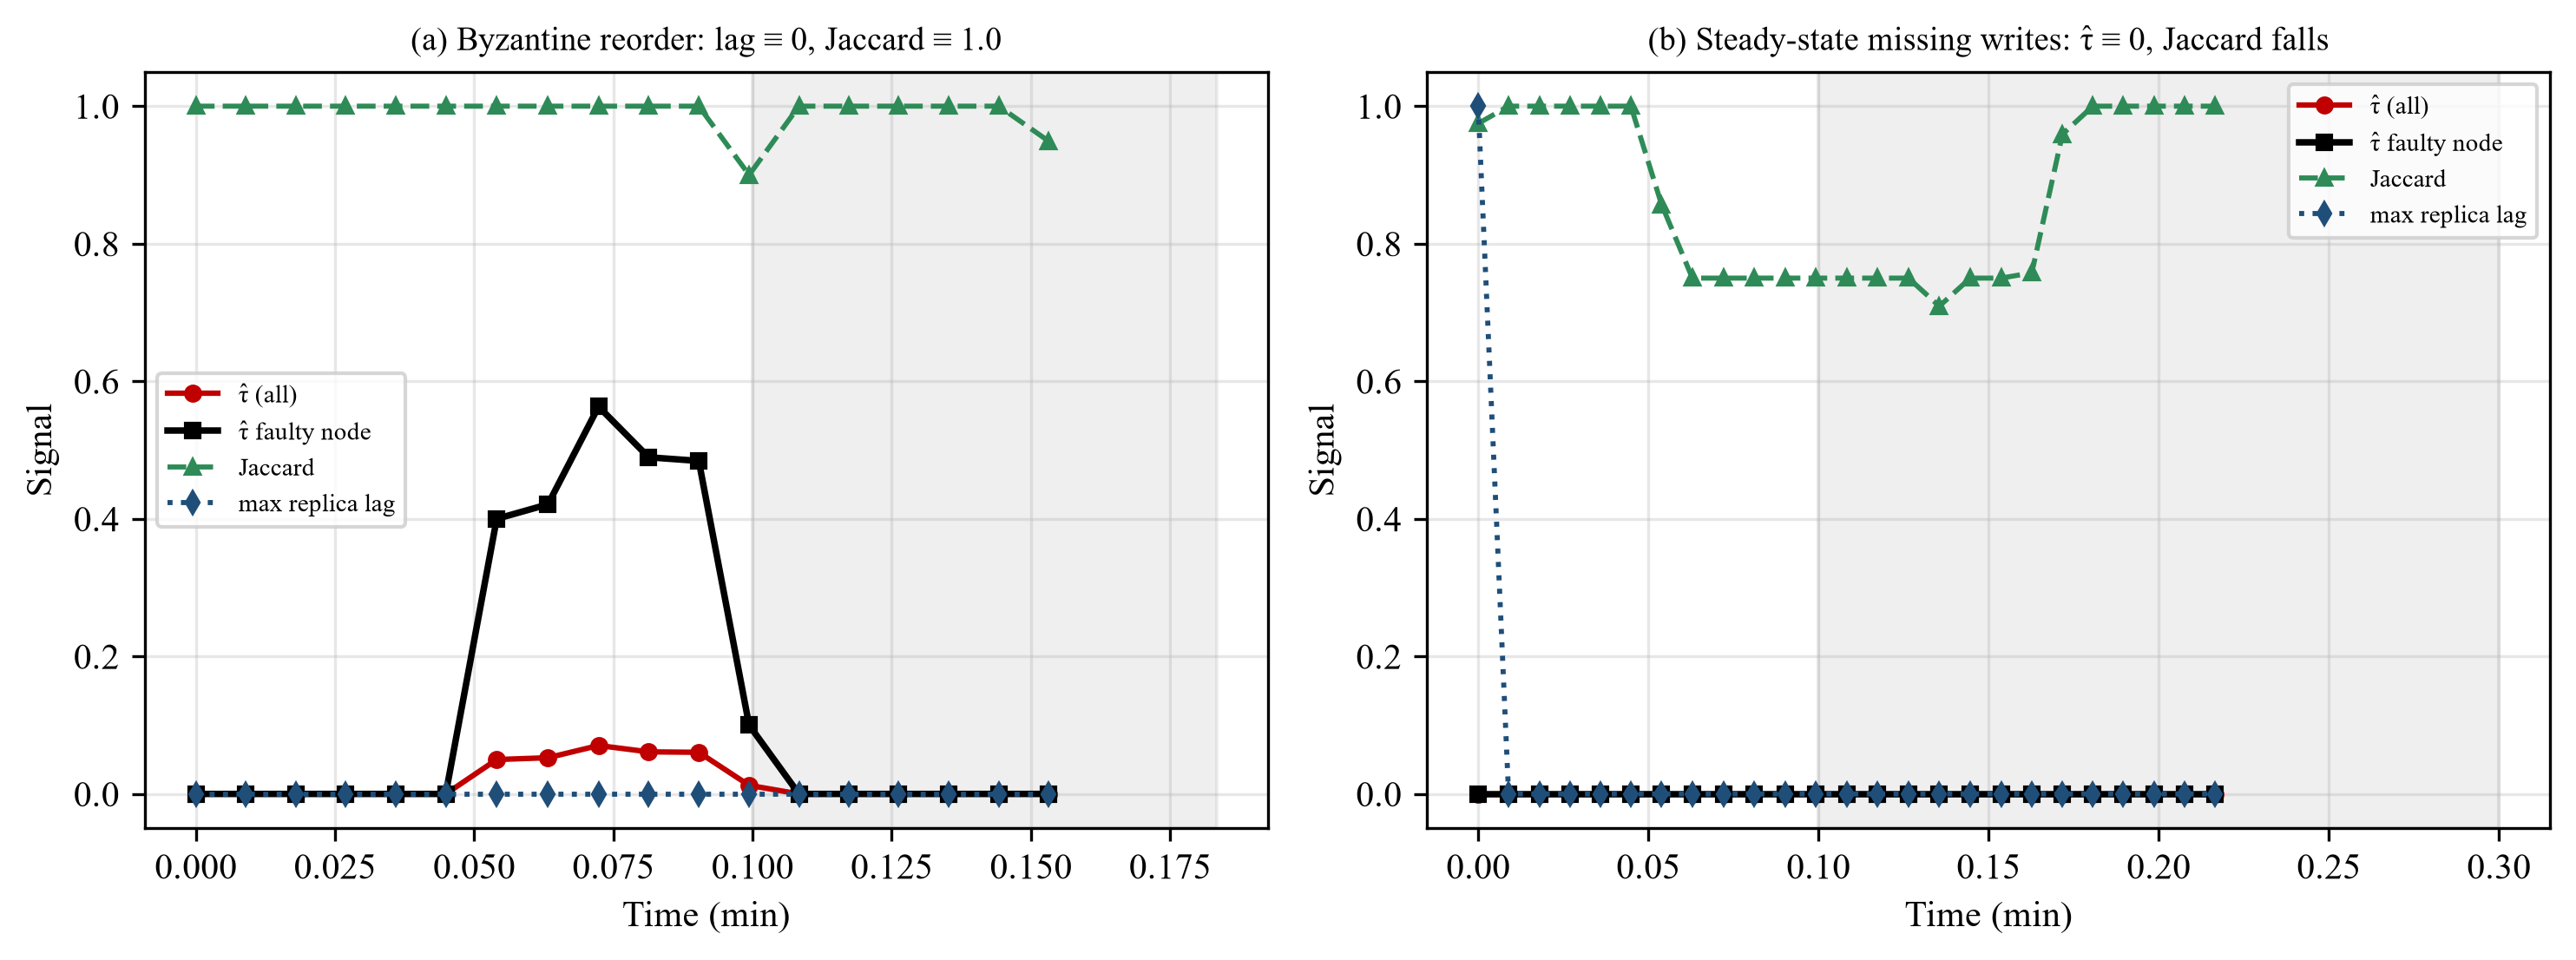
\includegraphics[width=0.95\textwidth]{figures/fig7.png}
\caption{Fig. 7. Fault-injection monitoring on the Cassandra cluster (E7). (a) Byzantine reorder: $\hat{\tau}$ rises and the faulty replica's per-node $\hat{\tau}$ dominates while lag $\equiv$ 0 and Jaccard $\equiv$ 1.0. (b) Steady-state missing writes: $\hat{\tau}$ $\equiv$ 0 while Jaccard falls—set-level faults are invisible to $\tau$ and caught by the Jaccard/repair signals. Shaded region: fault window.}
\end{figure}

\begin{table}[t]
\centering
\caption{Table 6. Fault-injection evaluation (E7) on the Cassandra cluster: detection latency and faulty-replica localization. —” = never detected; localization reports the fraction of fault-window samples in which the faulty replica ranks first (per-replica $\hat{\tau}$; Jaccard/repair = set-mismatch signal). Means over 3 trials.}
\begin{tabular}{llllllll}
\hline
Scenario (fault) & $\hat{\tau} detect (s)$ & lag detect (s) & Jaccard detect (s) & $\hat{\tau} loc.$ & Jaccard/repair loc. & Steady false alarms & $Peak \hat{\tau} (faulty)$ \\
\hline
S1 partition + reorder & 0.47 & — & 0.28 & 0.12 & 1.00 & 0 & 0.31 \\
S2 Byzantine reorder & 0.55 & — & — & 1.00 & blind & 0 & 0.61 \\
S3 Byzantine phantom & — & — & 0.35 & blind & 1.00 & 0 & 0.00 \\
S4 steady missing & — & — & 0.38 & blind & 1.00 & 0 & 0.00 \\
\hline
\end{tabular}
\end{table}

\subsection{Comparison with the Theoretical Model}
\begin{table}[t]
\centering
\caption{Table 5. Live monitoring (E4): detection of ordering drift invisible to binary lag and operation-set similarity.}
\begin{tabular}{llllllll}
\hline
$drift_{\mathrm{max}}$ & Detect delay (s) & maxlag @detect & Steady false alarms & $Peak \hat{\tau} (drift)$ & $Peak \hat{\tau} (partition)$ & Jaccard min (partition) & Jaccard @heal \\
\hline
0.10 & 1.297 & 0 & 0 & 0.305 & 0.000 & 0.408 & 0.949 \\
0.20 & 0.134 & 0 & 0 & 0.381 & 0.000 & 0.405 & 0.976 \\
0.40 & 1.191 & 0 & 0 & 0.400 & 0.000 & 0.429 & 0.810 \\
0.60 & 1.134 & 0 & 0 & 0.435 & 0.000 & 0.429 & 0.949 \\
\hline
\end{tabular}
\end{table}

\section{Practical Feasibility}
We briefly sketch how $\tau$-based reconciliation integrates into a recovery pipeline and confirm that its cost is negligible.

\subsection{Reconciliation Pipeline}
Upon partition healing, the framework prescribes: (1) collect the divergent logs with their version-clock contexts and derive the union happens-before DAG P—no propagation round is performed; (2) partition operations into conflict groups via vector-clock comparison (union-find); (3) for each group, apply a $\tau$-oriented merge—our validated instantiation is the lexicographic case of weighted Ranked Pairs (Proposition 4(a)): lock the causal edges of P with infinite penalty, compute pairwise margins over the partial ballots, lock majority-margin edges while the graph stays acyclic, and output a topological order; (4) concatenate the groups in causal order with the common prefix; (5) run the $O(M^{2})$ verification scan of Proposition-2 arithmetic to confirm no causal edge is inverted (guaranteed by step 3, retained as a runtime assertion); and (6) direct all replicas to roll back to the common-prefix snapshot and replay the merged log. The framework itself is method-agnostic: the objective $(\tau$ over feasible merges) and the causal check come from the measurement theory, and production systems may substitute any $\tau$-oriented method; because feasibility is imposed by the constraint set rather than assumed of the ballots, causal validity holds unconditionally—partial observation, missing ballots, and lossy delivery degrade contested-pair precision, never causal correctness.

\subsection{Recovery Cost}
\begin{table}[t]
\centering
\caption{Table 7. Recovery-time breakdown for a large conflict group (M = 50, N = 10). Ranking time is measured (Fig. 6); the remaining phases are estimated for a typical in-memory state machine.}
\begin{tabular}{lll}
\hline
Phase & Time (ms) & Fraction \\
\hline
Log collection & 0.50 & 9.9\% \\
Conflict detection & 0.12 & 2.4\% \\
Ranking (Ranked Pairs) & 4.45 & 87.7\% \\
Total (excluding replay) & 5.07 & 100\% \\
\hline
\end{tabular}
\end{table}

Rollback-and-replay cost depends on the state machine: for an in-memory store it is negligible, whereas for persistent stores it scales with the number of replayed operations and typically dominates total recovery time. Even for an unusually large group of 50 operations, the reconciliation-specific cost is under 15 ms; for realistic groups (M < 15), ranking is under 1 ms (Fig. 6), negligible against replay and network costs. The $\tau$-guided approach is thus computationally practical.

\section{Discussion}
\subsection{Threats to Validity}
The theoretical results (Propositions 1–4) hold for any input and are established by proof; Proposition 4(a)'s causal guarantee rests on the constraint set—the happens-before DAG from version-clock metadata—not on any premise about the ballots. A residual threat remains: if some happens-before edges were never recorded (e.g., lossy context propagation), the derived DAG under-approximates causality; the §8.1 verification scan checks feasibility against the derived DAG but cannot detect edges absent from the metadata.

\subsection{Why Not Just Use Causal Validity?}
Causal validity alone is insufficient as a quality standard because it is binary and coarse. Both a majority-respecting merge and an alphabetically sorted yet causally valid merge pass the test, yet they differ dramatically in how faithfully they preserve observed histories. Kendall $\tau$ fills this gap by measuring the continuous ordering-quality spectrum between causal validity and perfect agreement—a metric, not just a correctness condition, is needed.

\subsection{Relation to Rank Aggregation}
We borrow Kendall tau from social choice and computational social choice, where it is the canonical distance measure for rank aggregation [10], [20]. The rank-aggregation literature provides the theoretical machinery—Kemeny-Young optimality, Condorcet consistency, approximation algorithms—our application builds on. Our contribution is not a new voting rule but the identification of Kendall $\tau$ as the right quality metric for diverged log reconciliation, the causal-decomposition result connecting $\tau$ to distributed-systems correctness, and the unifying analysis of the reconciliation design space.

\subsection{Future Work}
Three directions stand out: weighted $\tau$ accounting for operation importance (Section 9.4.1); larger-scale deployment on production traces (the preliminary validation of Section 7 leaves scale and trace diversity open); and online monitoring—Section 7 provides the first experimental confirmation that $\tau$ detects ordering-only divergence invisible to binary lag and that combining $\tau$ with operation-set Jaccard similarity disambiguates degraded from fully partitioned phases, leaving adaptive thresholds and distributed monitor deployment open.

\subsubsection{Weighted Kendall $\tau$: Accounting for Operation Importance}
The unweighted $\tau$ treats every operation pair equally, but operations carry heterogeneous importance. The weighted distance $\tau_{w}(\sigma)$ = $\sum_{i}$ $\sum_{(a,b)\in L_{i}}$ $w_{\mathrm{ab}}$ $\cdot$ 1[a $\succ\sigma$ b $\wedge$ b $\succ$ Li a] assigns a nonnegative weight $w_{\mathrm{ab}}$ per pair $(w_{\mathrm{ab}}$ $\equiv$ 1 reduces to $\tau);$ pairwise-weighted Kendall correlations [47] and weighted Kemeny aggregation [48] are studied in the ranking literature. Because weights factor out of per-pair contributions, the weighted distance remains a proper metric for symmetric w, and the weighted majority relation on a pair is decided by $\sum_{i}$ $w_{\mathrm{ab}}$ (1[a $\succ$ Li b] $-$ 1[b $\succ$ Li a]).

Applications. (i) Operation criticality: weight non-commutative operations (set, cas) above commutative increments, so ordering quality concentrates where order actually matters. (ii) Key heat: weight pairs by the access frequency of their key, emphasizing contended hot keys over cold ones. (iii) Recency: apply a time-decay weight so recent operations dominate the score, reflecting that ordering quality matters most immediately after healing. (iv) Replica authority: weight each replica's votes by its role (e.g., quorum weights under RF configurations), so minority observers contribute less.

Implementation path. The weighted objective replaces margins by weighted margins $m_{w}(a,$ b) = $\sum_{i}$ $w_{\mathrm{ab}}$ (1[a $\succ$ Li b] $-$ 1[b $\succ$ Li a]), after which Ranked Pairs runs unchanged in $O(M^{2}$ log M); the effective normalization generalizes to $Z_{\mathrm{eff}}(w)$ = $\sum_{i}$ $\sum_{(a,b)\in L_{i}}$ $w_{\mathrm{ab}}.$ Weights can be calibrated from domain priors (operation types) or telemetry (key heat, replica load). Validation would extend Section 6's metrics to weighted variants with a sensitivity analysis over weight settings; we leave the weighted decomposition theory and its empirical study to future work.

Weighted Ranked Pairs: making aggregation robust to partial observation. The concrete threat to Condorcet-style aggregation on partial ballots is that a causal edge can be outvoted. Under complete ballots every causal pair has margin N—the maximum possible—and cannot be part of a majority cycle (a cycle requires each edge to be majority-supported, while a causal pair is supported by every observer), so no Condorcet-consistent method inverts it; under partial observation the margin of a causal pair falls below N, and an opposing cycle of contested pairs with larger margins can override it—the 37.5\% violation rate of unweighted Ranked Pairs on our trace scenarios (§7). The fix is to weight causal edges: assign each causal pair (a, b) a penalty w > 0 on the inversion b $\succ$ a and run Ranked Pairs with weighted margins. The guarantee is exact when the penalty is infinite (lexicographic priority)—the instantiation validated in §6.2—and holds for finite w exactly when w exceeds the maximum total weight of any opposing cycle through the pair, a workload-dependent condition. Future work comprises: (i) calibrating finite weights from semantic cost (the damage of a causal inversion) or telemetry, trading strict causality for contested-pair quality where the application allows; (ii) a sensitivity analysis over w from 1 to $\infty$ mapping the causal-violation rate and retention frontier; and (iii) the Condorcet-paradox analysis above—when no Condorcet winner exists among contested pairs, characterizing which causal inversions a bounded-weight rule can still be forced to make, and the minimal weight that prevents them.

\section{Conclusion}
This paper proposes Kendall tau distance as a quality metric for diverged log reconciliation—a domain where strategies have traditionally been compared only qualitatively. Pairwise inversions turn out to be a unifying primitive: availability, causal validity, ordering fidelity, and automation are all aspects of how a system manages ordering disagreements, and $\tau$ puts them on a common scale. The causal-decomposition theorem gives this structure: total $\tau$ splits into a causal component (which any correct reconciler must drive to zero) and a contested component (which measures the genuine disagreement that remains after causality is satisfied). This provides a precise formulation of order quality that goes beyond the binary yes/no of causal consistency: feasibility under the causal partial order guarantees the causal component at zero cost, and the contested component—which only feasible merges trade—is what $\tau$ optimizes. Causal validity is necessary but not sufficient, and $\tau$ captures how much ordering quality remains.

Viewed through this metric, each reconciliation strategy appears as a design decision with a measurable price: leader overwrite's retention law, LWW's coordination-free retention loss, vector clocks' deferral penalty, CRDTs' commutativity boundary, and $\tau-aggregation's$ computation-cost exchange. $\tau$-minimization defines the order-optimality frontier—where operations do not commute, the order minimizing total pairwise disagreement best agrees with the collective observations—and CRDTs define the complementary order-irrelevance ceiling where no ordering decision is needed at all.

The measurement framework itself is the paper's contribution, and its algorithmic content is deliberately modest. One concrete instantiation—the lexicographic case of weighted Ranked Pairs, which locks causal edges with infinite penalty—demonstrates that $\tau$-optimal feasible merging is practically achievable: within 0.35\% on average of the constrained Kemeny-Young optimum (exact in 89\% of synthetic and 100\% of trace trials), with causal validity guaranteed by construction and sub-millisecond cost for realistic conflict groups—in sharp contrast to plain unweighted aggregation, which violates causal constraints on real traces in 37.5\% of trials. The framework's premises are explicit: under complete ballots the $\tau$-optimal merge is the Condorcet-consistent consensus order; under partial observation the effective normalization keeps measurement meaningful, and principled aggregation becomes the open problem. The framework also ships as an operational artifact: the monitoring system of §7 is the ordering-axis component of divergence monitoring—it detects and localizes ordering corruption that replica-lag and similarity signals cannot see (verified on real traces and a real cluster), while set-level divergence is left to the complementary Jaccard and repair signals, per the two-axis decomposition of §5.5. Generalizing the weighting—finite, calibrated penalties on causal-inverting orderings, together with an analysis of when Condorcet-paradox cycles can force causal inversions and how large penalties must be to prevent them (§9.4.1)—is the natural continuation that extends rank aggregation to all observation regimes.

\begin{thebibliography}{48}
\appendix
\section*{Appendix A}
\subsection{A.1 Platform and Implementation}
The real-trace validation ran on a four-node Cassandra 4.1 cluster (RF = 2) deployed with Docker Compose on a single host—one CPU and 1 GB heap per node, 2.0 CPU / 3 GB container limits, official cassandra:4.1 image, production defaults. A Python coordinator (cassandra-driver, 127.0.0.1:9042) reads per-replica logs and runs all strategies on identical inputs. BGL (LLNL) and HDFS (Hadoop) traces from the Loghub mirror [44] were parsed into typed operations; 2,000 log lines per dataset were imported (438 ops/s). CQL round-trip latency was p50 2.2 / p95 3.1 / p99 3.5 ms; cluster CPU averaged 2.5\% (peak 40\%) with 1.5 GB memory per node, so the platform contribution to reported timings is negligible.

\subsection{A.2 Scenario Generation and Fairness Protocol}
Each log line maps to an operation under the semanticization of §6.1: the issuing node is hashed to one of N = 8 logical replicas (mapped onto the 4 physical nodes); the line timestamp becomes the operation timestamp (the LWW basis); and the Level/Label field determines the type $(INFO\rightarrowcommutative$ incr; $WARN/ERROR\rightarrowset;$ $FATAL/SEVERE/alert\rightarrowconditional$ cas). A causal DAG is constructed from within-node temporal adjacency plus probabilistic cross-node edges, with the cross-edge probability tuned by binary search to match the target causal density; M = 24 operations are sampled per trial into one connected conflict group, each replica's log being a causally consistent subsequence with clock skew bounded at 500 $\mu$s and 5\% observation noise, used directly as the partial ballot (obs $\approx$ 0.9); the random seed is fixed at 42.

\subsection{A.3 Raw Results}
\begin{table}[t]
\centering
\caption{Table A1. CF-RP vs. the causally constrained Kemeny-Young optimum on trace-driven scenarios (N = 8, 24 trials per size): CF-RP is exact in 100% of trials at every size, with zero excess and zero violations of any causal constraint; unconstrained Ranked Pairs over the same partial ballots violates causal edges in 37.5% of trials.}
\begin{tabular}{lllll}
\hline
M & RP exact (\%) & $Avg. \tau / opt.$ & Max excess & Interpretation \\
\hline
5 & 100\% & 100.0\% & 0.0\% & Exact + causally valid in all trials \\
6 & 100\% & 100.0\% & 0.0\% & Exact + causally valid in all trials \\
7 & 100\% & 100.0\% & 0.0\% & Exact + causally valid in all trials \\
8 & 100\% & 100.0\% & 0.0\% & Exact + causally valid in all trials \\
\hline
\end{tabular}
\end{table}

\begin{table}[t]
\centering
\caption{Table A2. End-to-end quality on trace scenarios (E2, high conflict, N = 8, M = 24, 30-trial means, partial ballots, no dissemination). Ops ret. = operations retained; Info ret. = 1 $-$ $\hat{\tau}$. CF-RP recovers the exact consensus order (100.0%); LWW, CRDT, and CRDT+LWW follow at 99.0% (p = 0.008 vs. CF-RP); vector clocks defer contested decisions to random tie-breaking and fall significantly behind (68.4%, p < 0.001).}
\begin{tabular}{llllllll}
\hline
Strategy & Ops ret. & Auto cov. & Info ret. & Caus. viol. & Sem. valid. & Gini & Time (ms) \\
\hline
Leader overwrite & 60.7\% & 100\% & 99.5\%* & 0.0 & 88.4\% & 0.146 & 0.011 \\
LWW & 100\% & 100\% & 99.0\% & 0.0 & 82.2\% & 0.258 & 0.022 \\
Vector clocks & 100\% & 90.8\% & 68.4\% & 0.0 & 79.1\% & 0.676 & 0.045 \\
Pure CRDT & 100\% & 90.8\% & 99.0\% & 0.0 & 82.2\% & 0.258 & 0.025 \\
CRDT + LWW fb. & 100\% & 100\% & 99.0\% & 0.0 & 82.2\% & 0.258 & 0.016 \\
Ranked Pairs & 100\% & 100\% & 100.0\% & 0.0 & 82.8\% & 0.000 & 0.312 \\
\hline
\end{tabular}
\end{table}

* On the 50.3\% of operations retained. $\tau_{\mathrm{causal}}$ = 0 for every strategy, both conflict levels, all 30 trials. Ranked Pairs, LWW, and CRDT output identical orders on every trial (pairwise tied, p = 1.0), because the trace's single-source timestamps resolve concurrent pairs identically to the majority vote; vector clocks differ only in their random tie-breaking and lose 30.3 points of ordering information to it.

\begin{table}[t]
\centering
\caption{Table A3. Partition asymmetry (E6a) with partial ballots: operations retained and ordering information retained as the minority partition grows from 10% to 50%.}
\begin{tabular}{lllll}
\hline
Minority share & Leader ops ret. & LWW info ret. & RP info ret. & $RP \hat{\tau}$ \\
\hline
10\% & 90.0\% & 67.5\% & 77.5\% & 0.225 \\
20\% & 79.2\% & 67.8\% & 77.3\% & 0.227 \\
30\% & 68.9\% & 69.6\% & 78.0\% & 0.220 \\
40\% & 58.1\% & 69.3\% & 77.9\% & 0.221 \\
50\% & 50.8\% & 69.0\% & 77.7\% & 0.223 \\
\hline
\end{tabular}
\end{table}

\begin{table}[t]
\centering
\caption{Table A4. Computational cost on the trace platform with partial ballots (p50 over trials) and cluster resource utilization (docker stats sampling mean).}
\begin{tabular}{lllll}
\hline
M & $\tau_{\mathrm{total}} (ms)$ & Ranked Pairs (ms) & Merge throughput (ops/s) & Cluster CPU / mem \\
\hline
5 & 0.005 & 0.020 & 245,387 & $\approx$2.5\% / 1.5 GB per node \\
20 & 0.022 & 0.221 & 90,652 & CQL p50 = 2.2 ms \\
50 & 0.054 & 1.513 & 33,044 & CQL p95 = 3.1 ms \\
100 & 0.240 & 24.647 & 4,284 & CQL p99 = 3.5 ms \\
\hline
\end{tabular}
\end{table}

\begin{figure}[t]
\centering
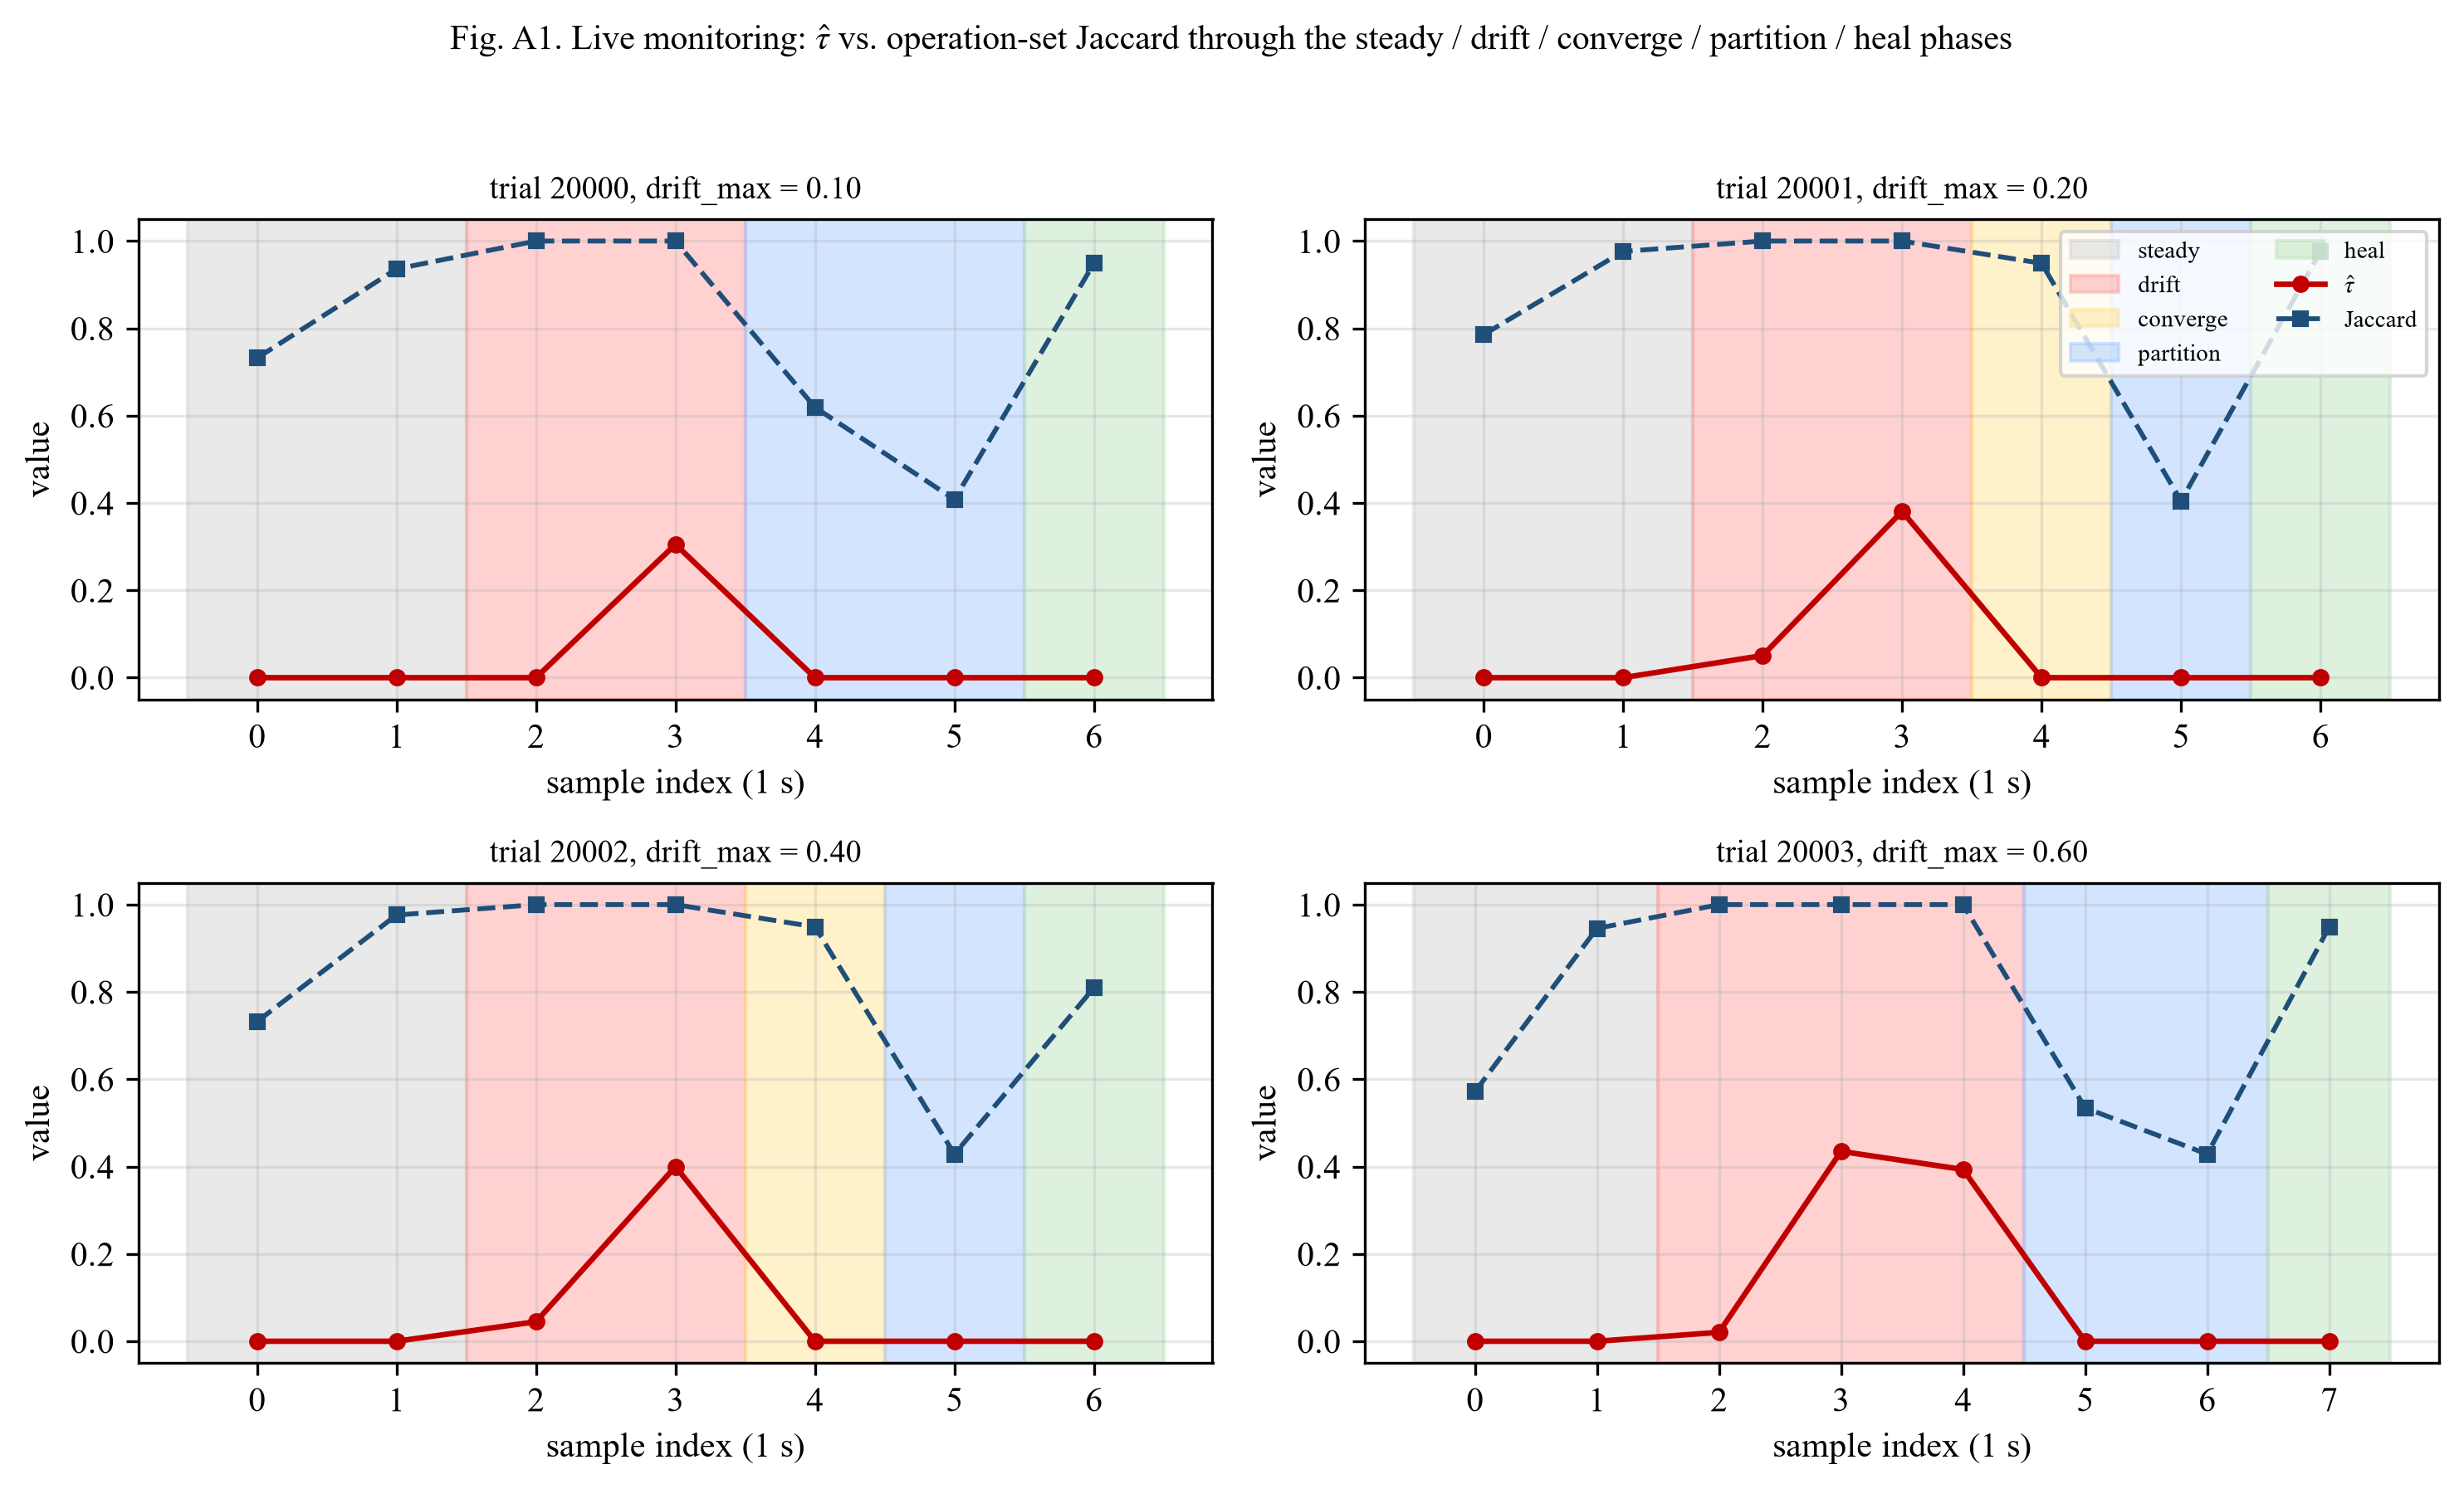
\includegraphics[width=0.95\textwidth]{figures/fig8.png}
\caption{Fig. A1. Live $\hat{\tau}$ and Jaccard trajectories through the five phases (one trial per drift strength). During drift, $\hat{\tau}$ rises while maxlag $\equiv$ 0 and Jaccard $\equiv$ 1.0; during partition, Jaccard falls while $\hat{\tau}$ $\approx$ 0: the two signals respond in disjoint failure modes.}
\end{figure}

\subsection{A.4 Reproducibility}
The complete suite—Docker Compose topology, trace files, scenario generator, strategies, monitor, and all raw per-trial CSVs—is archived with the project. Random seeds are fixed (42), and every CSV row is per-trial, so all tables in Section 7 and this appendix can be regenerated by re-running the pipeline: docker compose up -d; python \texttt{ingest\_trace.py};$ python \texttt{run\_experiments.py};$ python \texttt{analyze\_results.py}.$

The implementation and all experiment code are available from the authors upon request

\subsection{A.5 Statistical Details}
Statistics are computed per-trial over paired inputs (identical scenario and seed per trial); means are reported with standard deviations, 95\% confidence intervals use the t distribution with n $-$ 1 degrees of freedom, and pairwise significance uses the two-sided paired Wilcoxon signed-rank test at $\alpha$ = 0.05. Full per-metric tables for E1/E2/E6a (synthetic and trace) are archived in results/statistics\_*.csv.

\begin{table}[t]
\centering
\caption{Table A5. Synthetic E2 (N = 10, M = 24, n = 15, partial ballots obs = 0.9, no dissemination): ordering-information retention (1 $-$ $\hat{\tau}$) by strategy—mean $\pm$ std, 95% CI, and two-sided Wilcoxon p versus CF-RP.}
\begin{tabular}{llll}
\hline
Strategy & Mean $\pm$ std (\%) & 95\% CI (\%) & p vs. RP \\
\hline
Leader overwrite & 96.6 $\pm$ 1.4 & 95.8–97.4 & <0.001 \\
LWW & 67.5 $\pm$ 3.7 & 65.4–69.5 & <0.001 \\
Vector clocks & 61.3 $\pm$ 5.1 & 58.5–64.1 & <0.001 \\
Pure CRDT & 72.3 $\pm$ 3.3 & 70.5–74.2 & <0.001 \\
CRDT + LWW fb. & 67.5 $\pm$ 3.7 & 65.4–69.5 & <0.001 \\
Ranked Pairs & 76.8 $\pm$ 2.7 & 75.3–78.3 & — \\
\hline
\end{tabular}
\end{table}

LWW and CRDT+LWW produce identical outputs on every trial (p = 1.0); the LWW–VC difference is attributable to contested-deferral rather than causal failures, and the ranking on retention—CF-RP > pure CRDT > LWW > VC—holds with pairwise significance at $\alpha$ = 0.05.

\begin{table}[t]
\centering
\caption{Table A6. Trace E2 (N = 8, M = 24, n = 30, partial ballots, no dissemination): ordering-information retention by strategy—mean $\pm$ std, 95% CI, and two-sided Wilcoxon p versus CF-RP.}
\begin{tabular}{llll}
\hline
Strategy & Mean $\pm$ std (\%) & 95\% CI (\%) & p vs. RP \\
\hline
Leader overwrite & 99.5 $\pm$ 1.2 & 99.0–99.9 & 0.042 \\
LWW & 99.0 $\pm$ 1.7 & 98.3–99.6 & 0.008 \\
Vector clocks & 68.4 $\pm$ 8.7 & 65.2–71.7 & <0.001 \\
Pure CRDT & 99.0 $\pm$ 1.7 & 98.3–99.6 & 0.008 \\
CRDT + LWW fb. & 99.0 $\pm$ 1.7 & 98.3–99.6 & 0.008 \\
Ranked Pairs & 100.0 $\pm$ 0.0 & 100.0–100.0 & — \\
\hline
\end{tabular}
\end{table}

* On the trace platform CF-RP achieves retention 100.0 $\pm$ 0.0\% (identical on every trial), significantly above LWW / pure CRDT / CRDT+LWW (99.0 $\pm$ 1.7\%, p = 0.008) and vector clocks (68.4 $\pm$ 8.7\%, p < 0.001). Leader overwrite retains 60.7\% of operations; its 99.5\% retention applies to the surviving set. Unconstrained Ranked Pairs on the same ballots violates causal edges in 37.5\% of Table A1 trials. Gini and per-metric statistics for E1/E6a are in $results/statistics_{\mathrm{synthetic}}_{\mathrm{cf}}.csv$ and $results/statistics_{\mathrm{trace}}_{\mathrm{cf}}.csv.$

\section*{Appendix B}
\subsection{B.1 Effective Normalization}
The effective normalization $Z_{\mathrm{eff}}$ = $\sum_{i}$ $|Li|(|Li|-1)/2$ counts, per replica, exactly the pairs on which it can express an opinion; $\tau(\sigma,$ Li) counts only pairs present in Li and inverted relative to $\sigma,$ so $\hat{\tau}(\sigma)$ $\in$ [0, 1]. Under full observation $Z_{\mathrm{eff}}$ = $N\cdotM(M-1)/2$ and $\hat{\tau}$ matches the unnormalized definition; replicas with |Li| $\leq$ 1 contribute no pairs, and $Z_{\mathrm{eff}}$ = 0 only when no replica holds two operations.

\subsection{B.2 Proof of Proposition 1}
For $\sigma$ and its reverse $\sigmarev,$ every pair observed by replica i is inverted in exactly one of the two rankings, so $\tau(\sigma)$ + $\tau(\sigmarev)$ = $Z_{\mathrm{eff}}$ and $\hat{\tau}(\sigma)$ + $\hat{\tau}(\sigmarev)$ = 1; hence $\hat{\tau}_{\mathrm{min}}$ $\leq$ 1/2. The bound is tight: a profile in which every pair is split evenly (n(a $\succ$ b) = n(b $\succ$ a)) has $\hat{\tau}(\sigma)$ = 1/2 for every $\sigma;$ the supremum $\hat{\tau}$ = 0 is attained when all replicas agree.

\subsection{B.3 Proof of Proposition 2}
By pairwise additivity, $\tau_{\mathrm{total}}(\sigma)$ = $\sum_{\mathrm{pairs}}$ $c_{\mathrm{ab}}(\sigma),$ where $c_{\mathrm{ab}}(\sigma)$ counts the replicas observing both a and b and disagreeing with $\sigma$ on their order; pairs absent from a replica's log contribute 0. Fixing a unanimous causal pair (a, b): every observing replica ranks a before b, so $c_{\mathrm{ab}}(\sigma)$ = $n_{\mathrm{ab}}$ $\cdot$ 1[b $\succ\sigma$ a]. Summing over causal pairs gives $\tau_{\mathrm{causal}},$ over the remaining pairs $\tau_{\mathrm{contested}},$ and $\tau_{\mathrm{total}}$ = $\tau_{\mathrm{causal}}$ + $\tau_{\mathrm{contested}}$ follows from the partition of pairs.

\subsection{B.4 Proof of Proposition 3 and the Partial-Observation Boundary}
Main claim. Under complete ballots, the (constrained) Kemeny optimum respects every unanimous pair—the classical Pareto/Condorcet property [23]: if a $\tau$-minimal feasible $\sigma$ placed b above a, swapping the pair reduces cost by $n_{\mathrm{ab}}$ + $\sum_{y}$ [s(a,y) + s(y,b)] $\geq$ $n_{\mathrm{ab}}$ > 0 (every observer of a also observes b), a contradiction. Under partial observation the argument fails when a replica observes exactly one of a, b (contributions of $-1$ enter), and unconstrained aggregation can reverse a unanimous causal pair—feasibility enforcement (§5.3.2) is therefore necessary for soundness.

Boundary. Counterexample (causally consistent logs over {0, 1, 2, 3} with constraint 0 $\rightarrow$ 2): [3, 1, 0, 2], [3, 2, 1], [2, 3, 1]. Pair (0, 2) is unanimous among its single observer (0 before 2), yet unconstrained Kemeny optima include (3, 2, 1, 0), placing 2 above 0 (all optima have $\tau_{\mathrm{total}}$ = 3); the feasible optima all place 0 before 2, and CF-RP never violates the pair. On our synthetic workloads the constraint binds rarely (constrained = unconstrained optimum in 100\% of §6.2 trials), but on trace scenarios unconstrained Ranked Pairs violates causal edges in 37.5\% of trials (Table A1) at average quality cost 0.35\% (§6.2).

\subsection{B.5 Proof of Proposition 4}
(a) CF-RP locks every causal edge of P before any majority lock (margin +$\infty$); the union happens-before DAG is acyclic, so all locks succeed and the output is a linear extension of causal order for arbitrary partial ballots, without dissemination. Unconstrained Ranked Pairs has no such guarantee: under partial observation a unanimous pair has margin $n_{\mathrm{ab}}$ < N and can be outranked by larger-margin pairs, as in the profile [1, 0, 2, 3], [1, 3, 0], [3, 0, 1] with constraint 0 $\rightarrow$ 2 (§B.4). Schulze and Copeland admit the identical constraint—fix causal edges before running the method.

(b) In the full-information setting a unanimous pair gives every voter a strictly higher Borda score to a, so the aggregate difference is at least $n_{\mathrm{ab}};$ with partial observation, voters observing exactly one of the two flip the difference—the same boundary as (a). (c) The local-search counterexample of §5.3.3 shows the failure for heuristics: the adjacent-swap local optimum $\sigma$ = b $\succ$ z$_{1}$ $\succ$ z$_{2}$ $\succ$ a violates the unanimous pair (a, b) with $\tau_{\mathrm{causal}}$ = $n_{\mathrm{ab}}$ = 3, which Proposition 2 counts exactly; Kemeny-optimal rankings do not exhibit this failure under the conditions of Proposition 3, but timestamps and local search offer no guarantee.

\bibitem{1} L. Lamport, "The part-time parliament," ACM Transactions on Computer Systems, vol. 16, no. 2, pp. 133–169, 1998.
\bibitem{2} L. Lamport, "Paxos made simple," ACM SIGACT News, vol. 32, no. 4, pp. 18–25, 2001.
\bibitem{3} J. Bartholdi, C. Tovey, and M. Trick, "Voting schemes for which it can be difficult to tell who won the election," Social Choice and Welfare, vol. 6, no. 2, pp. 157–165, 1989.
\bibitem{4} N. Tideman, "Independence of clones as a criterion for voting rules," Social Choice and Welfare, vol. 4, no. 3, pp. 185–206, 1987.
\bibitem{5} M. Schulze, "A new monotonic, clone-independent, reversal symmetric, and Condorcet-consistent single-winner election method," Social Choice and Welfare, vol. 36, no. 2, pp. 267–303, 2011.
\bibitem{6} J.-C. de Borda, "Mémoire sur les élections au scrutin," Histoire de l'Académie Royale des Sciences, 1781.
\bibitem{7} A. H. Copeland, "A reasonable social welfare function," University of Michigan Seminar on Applications of Mathematics to the Social Sciences, 1951.
\bibitem{8} C. Dwork, R. Kumar, M. Naor, and D. Sivakumar, "Rank aggregation methods for the web," in Proc. 10th Int. Conf. World Wide Web (WWW), 2001, pp. 613–622.
\bibitem{9} G. DeCandia et al., "Dynamo: Amazon's highly available key-value store," in Proc. 21st ACM Symp. Operating Systems Principles (SOSP), 2007, pp. 205–220.
\bibitem{10} M. G. Kendall, "A new measure of rank correlation," Biometrika, vol. 30, no. 1–2, pp. 81–89, 1938.
\bibitem{11} J. G. Kemeny and J. L. Snell, Mathematical Models in the Social Sciences. Boston, MA: Ginn, 1962.
\bibitem{12} D. Ongaro and J. Ousterhout, "In search of an understandable consensus algorithm," in Proc. USENIX Annual Technical Conf. (ATC), 2014, pp. 305–319.
\bibitem{13} M. Shapiro, N. Preguiça, C. Baquero, and M. Zawirski, "Conflict-free replicated data types," in Proc. 13th Int. Symp. Stabilization, Safety, and Security of Distributed Systems (SSS), 2011, pp. 386–400.
\bibitem{14} I. Moraru, D. G. Andersen, and M. Kaminsky, "There is more consensus in egalitarian parliaments," in Proc. 24th ACM Symp. Operating Systems Principles (SOSP), 2013, pp. 358–372.
\bibitem{15} Y. Mao, F. P. Junqueira, and K. Marzullo, "Mencius: building efficient replicated state machines for WANs," in Proc. 8th USENIX Symp. Operating Systems Design and Implementation (OSDI), 2008, pp. 369–384.
\bibitem{16} J. C. Corbett et al., "Spanner: Google's globally distributed database," in Proc. 10th USENIX Symp. Operating Systems Design and Implementation (OSDI), 2012, pp. 251–264.
\bibitem{17} A. Lakshman and P. Malik, "Cassandra: a decentralized structured storage system," ACM SIGOPS Operating Systems Review, vol. 44, no. 2, pp. 35–40, 2010.
\bibitem{18} B. Reed and F. P. Junqueira, "A simple totally ordered broadcast protocol," in Proc. 2nd Workshop on Large-Scale Distributed Systems and Middleware (LADIS), 2008, Art. 2.
\bibitem{19} W. V. Gehrlein and P. C. Fishburn, "The Condorcet criterion and committee selection," Mathematical Social Sciences, vol. 1, no. 3, pp. 293–305, 1980.
\bibitem{20} F. Brandt, V. Conitzer, U. Endriss, J. Lang, and A. D. Procaccia, Eds., Handbook of Computational Social Choice. Cambridge, U.K.: Cambridge Univ. Press, 2016.
\bibitem{21} P. C. Fishburn, "Condorcet social choice functions," SIAM Journal on Applied Mathematics, vol. 33, no. 3, pp. 469–489, 1977.
\bibitem{22} H. P. Young, "Optimal voting rules," Journal of Economic Perspectives, vol. 9, no. 1, pp. 51–64, 1995.
\bibitem{23} H. P. Young and A. Levenglick, "A consistent extension of Condorcet's election principle," SIAM Journal on Applied Mathematics, vol. 35, no. 2, pp. 285–300, 1978.
\bibitem{24} G. Goren and D. Malkhi, "Making democracy work: fixing and simplifying egalitarian Paxos," arXiv preprint arXiv:2511.02743, 2025.
\bibitem{25} A. Ryabinin, R. Oshman, and I. Keidar, "SwiftPaxos: fast geo-replicated state machines," in Proc. 21st USENIX Symp. Networked Systems Design and Implementation (NSDI), 2024.
\bibitem{26} Y. Tang et al., "Jetpack: consensus made generally fast," in Proc. 22nd USENIX Symp. Operating Systems Design and Implementation (OSDI), 2026.
\bibitem{27} C. J. Fidge, "Timestamps in message-passing systems that preserve the partial ordering," in Proc. 11th Australian Computer Science Conf. (ACSC), 1988, pp. 56–66.
\bibitem{28} F. Mattern, "Virtual time and global states of distributed systems," in Proc. Workshop on Parallel and Distributed Algorithms, 1989, pp. 215–226.
\bibitem{29} W. Lloyd, M. J. Freedman, M. Kaminsky, and D. G. Andersen, "Don't settle for eventual: scalable causal consistency for wide-area storage with COPS," in Proc. 23rd ACM Symp. Operating Systems Principles (SOSP), 2011, pp. 401–416.
\bibitem{30} W. Lloyd, M. J. Freedman, M. Kaminsky, and D. G. Andersen, "Stronger semantics for low-latency geo-replicated storage," in Proc. 10th USENIX Symp. Operating Systems Design and Implementation (OSDI), 2012, pp. 313–328.
\bibitem{31} M. Zawirski et al., "SwiftCloud: fault-tolerant geo-replication integrated all the way to the client machine," in Proc. 6th USENIX Workshop on Hot Topics in Cloud Computing (HotCloud), 2014.
\bibitem{32} G. Litt, S. Lim, M. Kleppmann, and P. van Hardenberg, "Peritext: a CRDT for collaborative rich text editing," in Proc. 35th ACM Symp. User Interface Software and Technology (UIST), 2022.
\bibitem{33} L. Da and M. Kleppmann, "Moving elements in JSON CRDTs," in Proc. 10th Workshop on Principles and Practice of Consistency for Distributed Data (PaPoC), 2024.
\bibitem{34} V. Zamfir, M. Crocke, and O. Shasha, "A Datalog framework for conflict-free replicated data types," Theory and Practice of Logic Programming, vol. 24, no. 3, pp. 646–682, 2024.
\bibitem{35} J. Kuessner, R. Mogk, M. Wickert, and M. Mezini, "A study of crdt composition," in Proc. 13th ACM SIGPLAN Int. Symp. Scala, 2023, pp. 44–57.
\bibitem{36} H. M. N. Saad and M. B. Habib, "FabricCRDT: a conflict-free replicated datatypes approach to permissioned blockchains," in Proc. 7th Int. Conf. Networked Systems (NETYS), 2023.
\bibitem{37} E. Dufresne and M. Vojnovi\'c, "Decentralized ranking aggregation via gossip: convergence and robustness," arXiv preprint arXiv:2602.22847, 2026.
\bibitem{38} X. Wang et al., "Illuminating patterns of divergence: DataDios SmartDiff for large-scale data difference analysis," in Proc. ACM SIGMOD Int. Conf. Management of Data, 2025, pp. 1234–1247.
\bibitem{39} S. Liu, Q. Zhang, and Y. Li, "Temporal logical attention network for log-based anomaly detection in distributed systems," Sensors, vol. 24, no. 24, Art. 7949, 2024.
\bibitem{40} Z. Chen et al., "Cloud Atlas: efficient fault localization for cloud systems using language models and causal insight," arXiv preprint arXiv:2407.08694, 2024.
\bibitem{41} G. Ramseyer and A. Goel, "Fair ordering via streaming social choice theory," in Proc. 43rd ACM Symp. Principles of Distributed Computing (PODC), 2024, pp. 1345–1348.
\bibitem{42} M. Kelkar, S. Deb, S. R. Choudhury, S. Bag, and P. Kothapalli, "Aequitas: admission control for fair ordering in blockchain systems," in Proc. 2021 ACM SIGSAC Conf. Computer and Communications Security (CCS), 2021, pp. 2127–2142.
\bibitem{43} Y. Zhang, D. Lu, N. K. Sharma, G. Fanti, and P. Viswanath, "Themis: fair and efficient transaction ordering," arXiv preprint arXiv:2205.06771, 2022.
\bibitem{44} J. Zhu, S. He, P. He, J. Liu, and M. R. Lyu, "Loghub: A large collection of system log datasets for AI-driven log analytics," in Proc. 34th IEEE Int. Symp. Software Reliability Engineering (ISSRE), 2023, pp. 355–366.
\bibitem{45} A. J. Oliner and J. Stearley, "What supercomputers say: a study of five system logs," in Proc. IEEE/IFIP Int. Conf. Dependable Systems and Networks (DSN), 2007, pp. 575–584.
\bibitem{46} P. Bailis, S. Venkataraman, M. J. Franklin, J. M. Hellerstein, and I. Stoica, "Probabilistically bounded staleness for practical partial quorums," Proc. VLDB Endowment, vol. 5, no. 8, pp. 776–787, 2012.
\bibitem{47} S. Vigna, "A weighted correlation index for rankings with ties," in Proc. 24th Int. Conf. World Wide Web (WWW), 2015, pp. 1166–1176.
\bibitem{48} S. D. Dvoenko and D. O. Pshenichny, "Developing the Kemeny's weighted median for the rank aggregation problem," in Proc. 4th Int. Conf. Future Networks and Distributed Systems (ICFNDS), 2020, pp. 1–4.
\bibitem{49} E. Lee, N. Kim, C. Han, N. Shin, and I. Lee, “rPBFT: Reliable Practical Byzantine Fault Tolerance Mechanism for Faulty Distributed Networks,” IEEE Transactions on Big Data, vol. 12, no. 3, pp. 814–828, 2026.
\end{thebibliography}
\end{document}
